\documentclass[12pt, a4paper]{article}

% ============================================================
%  Preamble
% ============================================================
\usepackage[utf8]{inputenc}
\usepackage[T1]{fontenc}
\usepackage{lmodern}
\usepackage{microtype}
\usepackage{amsmath, amssymb, amsthm}
\usepackage{graphicx}
\usepackage{booktabs}
\usepackage{array}
\usepackage{longtable}
\usepackage{listings}
\usepackage{xcolor}
\usepackage{enumitem}
\usepackage{titlesec}
\usepackage{abstract}
\usepackage{caption}
\usepackage{float}
\usepackage[margin=2.8cm]{geometry}
\usepackage[backend=biber, style=numeric]{biblatex}
\usepackage{hyperref} % load last

\addbibresource{sample.bib}

% ------------------------------------------------------------
%  Hyperref
% ------------------------------------------------------------
\hypersetup{
    colorlinks=true,
    linkcolor=blue!60!black,
    urlcolor=blue!60!black,
    citecolor=green!50!black
}

% ------------------------------------------------------------
%  Section formatting
% ------------------------------------------------------------
\titleformat{\section}{\large\bfseries}{\thesection.}{0.6em}{}
\titleformat{\subsection}{\normalsize\bfseries}{\thesubsection}{0.6em}{}

% ------------------------------------------------------------
%  Listings: Lean 4
% ------------------------------------------------------------
\definecolor{codebg}{HTML}{F5F5F5}
\definecolor{codecomment}{HTML}{5C8A5C}
\definecolor{codekeyword}{HTML}{2E4DA0}
\definecolor{codestring}{HTML}{B5380C}
\definecolor{codehole}{HTML}{B00020}

\lstdefinelanguage{Lean4}{
  keywords={theorem, lemma, def, noncomputable, let, have, intro, intros,
             cases, induction, calc, exact, apply, refine, rw, simp, simp_all,
             ring, linarith, nlinarith, omega, decide, native_decide, norm_num,
             congr, obtain, fun, import, open, where, by, with, of, in,
             Type, Prop},
  keywordstyle=\color{codekeyword}\bfseries,
  emph={sorry},
  emphstyle=\color{codehole}\bfseries,
  comment=[l]{--},
  commentstyle=\color{codecomment}\itshape,
  stringstyle=\color{codestring},
  sensitive=true,
  morestring=[b]",
}

\lstset{
  language=Lean4,
  backgroundcolor=\color{codebg},
  basicstyle=\ttfamily\footnotesize,
  breaklines=true,
  frame=single,
  framerule=0.4pt,
  rulecolor=\color{gray!50},
  xleftmargin=1em,
  xrightmargin=1em,
  aboveskip=1em,
  belowskip=1em,
  numbers=left,
  numberstyle=\tiny\color{gray},
  numbersep=8pt,
  captionpos=b,
  showstringspaces=false,
  literate=
    {ℕ}{{$\mathbb{N}$}}1
    {ℂ}{{$\mathbb{C}$}}1
    {ℝ}{{$\mathbb{R}$}}1
    {ℤ}{{$\mathbb{Z}$}}1
    {∣}{{$\mid$}}1
    {¬}{{$\lnot$}}1
    {∀}{{$\forall$}}1
    {∃}{{$\exists$}}1
    {≤}{{$\le$}}1
    {≥}{{$\ge$}}1
    {≠}{{$\ne$}}1
    {≡}{{$\equiv$}}1
    {→}{{$\to$}}1
    {↦}{{$\mapsto$}}1
    {∈}{{$\in$}}1
    {∉}{{$\notin$}}1
    {‖}{{$\Vert$}}1
    {∮}{{$\oint$}}1
    {⊢}{{$\vdash$}}1
    {·}{{$\cdot$}}1
    {×}{{$\times$}}1
    {π}{{$\pi$}}1
    {α}{{$\alpha$}}1
    {ω}{{$\omega$}}1
    {√}{{$\surd$}}1
    {∅}{{$\emptyset$}}1
    {⟪}{{$\langle\!\langle$}}2
    {⟫}{{$\rangle\!\rangle$}}2
    {₀}{{$_0$}}1
    {₁}{{$_1$}}1
    {₂}{{$_2$}}1
    {₃}{{$_3$}}1
}

% ============================================================
\begin{document}

\title{\textbf{Strategy and Capability in Machine Formalisation \\
\large Measuring the Extent to Which Agentic Scaffolding Improves the
Proving Capacity of Language Models in Lean~4}}
\author{Mikael Bashir \\ \textit{M3R/02382080}}
\date{\today}

\maketitle

\begin{abstract}
\noindent
Language models exhibit strong informal mathematical reasoning yet struggle
with the syntactic and semantic discipline of proof assistants. A now-common
response is to wrap the model in \emph{strategy}: decomposition
orchestrators, blueprint-refinement loops, parallel sub-agents, retrieval
governors, and oversight watchers. This paper asks how much of the resulting
capability is attributable to that scaffolding, and how much to the
underlying model driven competently against a compiler. We report on
\emph{Leak}, an agentic theorem-proving architecture connecting language
models to Lean~4 through the Model Context Protocol, and on a strategy
registry of nineteen named configurations that differ only in prompt,
orchestration and tool budget while sharing an identical verification gate,
governance clock and toolchain --- an arrangement that permits controlled
comparison between proving styles rather than anecdote.

We make four contributions. First, we characterise the execution substrate
precisely, distinguishing the batch \emph{Language Server Protocol} discipline
of the certifying verifier from the \emph{read--eval--print} discipline of the
interactive Pantograph daemon, and describe a snapshot-based extension that
serves an unbounded population of logical proof states from a single resident
elaboration environment. Second, we document a design invariant forced by an
early failure in which an agent escaped its loop by hallucinating its own
verification: the only reachable success state is a compiler certificate, and
no model-authored prose is load-bearing. Third, we report production results
--- 219 of 220 problems in a public competition corpus formally verified,
approximately 7{,}500 lines of Lean~4 --- alongside a controlled evaluation on
FATE-X, a benchmark of 100 graduate-level algebra problems, under a
single-pass protocol with a 60-minute wall-clock cap and, for
refinement-based strategies, an 8-iteration ceiling. Fourth, and least
comfortably, we report that our strongest measured configuration is a
blueprint-refinement pipeline, that several elaborate decomposition
strategies underperform it, and that a deliberately minimal control --- one
agent, one compiler, no decomposition --- solved a problem on which four
successive decomposition architectures had failed.

We therefore resist the conclusion that strategy is uniformly beneficial. The
evidence supports a weaker and more specific claim: scaffolding that
tightens the feedback loop or bounds context reliably helps, whereas
scaffolding that adds coordination structure without adding information can
degrade performance relative to a competent flat baseline. We further argue
that all such measurements, including ours, are currently confounded by data
contamination of a kind that release-date arguments cannot dispel, since
FATE-X is explicitly assembled from textbooks, qualifying examinations and
research literature, and we propose a difficulty-matched statistical control
as partial mitigation.
\end{abstract}

\newpage
\tableofcontents
\newpage

% ============================================================
\section{Introduction}
% ============================================================

The application of artificial intelligence to formal theorem proving has
traditionally been hindered by the uncompromising constraints of proof
assistants such as Lean~4~\cite{demoura2021lean4}. Built on the Calculus of
Inductive Constructions,
Lean guarantees absolute correctness by enforcing a rigorous type theory in
which every theorem is a type and every proof a term of that type. While
frontier-scale models occasionally produce correct proof scripts zero-shot,
generalised models suffer hallucinated lemma names, brittle syntax, and an
inability to track complex mathematical state across deep contexts.

Machine-assisted theorem proving is a distinctive computational challenge
because the search space is unbounded: there is no universal decision
procedure for provability in the general case, and individual tactic
sequences can be arbitrarily long. Prominent industrial systems ---
DeepSeek-Prover-V2~\cite{deepseekproverv2},
AlphaProof~\cite{alphaproof2024} --- address this by scaling compute to
extremes: reinforcement-learning pipelines, millions of auto-formalised
problem variants, and deep exploration trees scored by learned value
functions. Such architectures presuppose effectively unlimited resources.

This paper describes a different trajectory, developed across two system
generations under the working name \emph{Leak}, and uses it to interrogate a
question that the field's rapid architectural elaboration has largely
outrun.

\subsection{The Research Question}
\label{sec:research-question}

A substantial fraction of recent engineering effort in machine formalisation
has gone not into models but into \emph{strategy}: the orchestration layer
that decides how a model is invoked, what it sees, how its work is divided,
and what it is permitted to conclude. Systems decompose theorems into
subgoal trees~\cite{deepseekproverv2, davis2025goedelspoetry}, maintain
blueprint graphs subjected to iterative refinement, dispatch parallel
sub-agents against isolated holes, ration library retrieval, and install
supervisory critics over the whole apparatus. The implicit hypothesis is
that scaffolding converts a general-purpose model into a competent
formaliser, and that more scaffolding converts it into a better one.

The first half of that hypothesis is well supported, and not only in this
domain: \textcite{zywot2025smallagents} report that tool augmentation yields
larger and more consistent gains than parameter scaling, with 4B-parameter
tool-using agents outperforming 32B-parameter tool-free baselines, while also
observing that additional deliberation is \emph{not} monotonically helpful ---
unrestricted reasoning frequently degrades tool orchestration. The second
half is far less well established. Comparisons across published systems
confound strategy with model, toolchain, compute budget and benchmark, so
the marginal contribution of any particular orchestration idea is rarely
isolated.

This paper therefore asks: \textbf{to what extent, and under what
conditions, does agentic strategy improve the proving capacity of language
models in Lean~4?} We approach it by holding everything else fixed. The
Leak orchestrator carries a registry of nineteen named strategies
(Section~\ref{sec:registry}) which differ \emph{only} in prompt,
orchestration topology and tool budget; the verification gate, the
wall-clock governor, the Lean and Mathlib pins, and the MCP tool surface are
common to all of them. Adding a strategy is adding an experimental arm, not
forking a system.

The two development generations map onto that question as follows.

\begin{enumerate}[leftmargin=*]
  \item \textbf{Generation One} (Sections~\ref{sec:gen1-arch}--\ref{sec:failure})
    asked how far a \emph{compact, inexpensive} model can be pushed when it is
    denied search trees and granted, instead, a tight, high-frequency feedback
    loop against the real compiler. The answer was: surprisingly far on short
    horizons --- and the architecture's own failure modes turned out to be as
    instructive as its successes.
  \item \textbf{Generation Two} (Sections~\ref{sec:gen2-arch}--\ref{sec:gen2-results})
    asked the complementary question: holding the feedback discipline fixed,
    what happens when the reasoning engine is a frontier model, the governance
    unit changes from invocation counts to wall-clock time, and decomposition
    is reintroduced --- but only in a form where \emph{every intermediate
    structure is itself compiler-verified}? The answer is a production system
    that has formally verified 219 of 220 problems in a public competition
    corpus, including theorems whose proofs formalise non-trivial analytic
    machinery from first principles.
\end{enumerate}

Both generations share one architectural constant: the reasoning engine is
decoupled from the execution environment via the Model Context Protocol
(MCP)~\cite{anthropic2024mcp}, the open standard introduced by Anthropic in
November 2024 for connecting AI systems to external tools over
JSON-RPC~2.0. MCP collapses the $N \times M$ integration problem ($N$ tools,
$M$ models, bespoke connectors for each pair) into a single contract, which
is precisely what allowed the second generation to swap its foundation model
--- from Grok to Claude --- without touching the formal environment, and what
makes the strategy registry a controlled instrument rather than a collection
of incomparable prototypes. The Lean toolchain itself is version-locked per
deployment (Lean~4 \texttt{v4.29.1} with a matching Mathlib pin for the
principal services; \texttt{v4.32.0} for the blueprint toolchain of
Section~\ref{sec:architect}), turning the proof environment into a
reproducible, interrogable service rather than a static corpus the model
must memorise.

\subsection{Summary of Findings}

We state the principal results here, and defer their qualification to
Sections~\ref{sec:results-fatex} and~\ref{sec:contamination}.

\begin{itemize}[leftmargin=*]
  \item \textbf{Scaffolding that tightens feedback or bounds context is
    reliably beneficial.} The compiler-certificate invariant, the retrieval
    governor, wall-clock governance, and the skeleton-first structural gate
    each removed a specific, observed failure mode, and the production
    corpus of Section~\ref{sec:gen2-results} was not attainable without them.
  \item \textbf{Scaffolding that adds coordination without adding
    information is not reliably beneficial.} Several elaborate
    decomposition strategies --- including two designed specifically to fix
    deficiencies observed in their predecessors --- did not outperform
    simpler configurations on the FATE-X subset we measured, and in some
    cases consumed an entire hour of wall clock without producing a
    certificate.
  \item \textbf{A minimal control is a stronger baseline than expected.}
    Two deliberately unsophisticated configurations --- a single agent, a
    single compiler, no decomposition and no give-up state --- each proved a
    problem on which four successive decomposition architectures had failed
    (Section~\ref{sec:control-observation}). We regard this as diagnostic of
    implementation defects in the decomposition family rather than as
    evidence against decomposition in principle, and say so explicitly.
  \item \textbf{Every one of these measurements is confounded by
    contamination.} FATE-X is assembled from textbooks, qualifying
    examinations and research literature~\cite{fatex2025}; the mathematics it
    tests is, by construction, material that any broadly-trained model has
    encountered. Section~\ref{sec:contamination} treats this at length rather
    than as a disclaimer.
\end{itemize}

% ============================================================
\section{Background: The Formal Verification Bottleneck}
% ============================================================

Three properties of the Lean~4~\cite{demoura2021lean4} +
Mathlib~\cite{mathlib2020} ecosystem shape every design
decision that follows.

\paragraph{Verification is binary and adversarial.} A proof either
type-checks or it does not. There is no partial credit, and the most
dangerous artefact an agent can produce is a script that \emph{looks}
correct: syntactically fluent, well-commented, and rejected by the kernel.
Any architecture that permits the model to assert its own success will
eventually be defeated by exactly this artefact (Section~\ref{sec:failure}).

\paragraph{The library is vast and its naming is adversarially irregular.}
Mathlib~\cite{mathlib2020} contains on the order of $10^5$ declarations whose naming
conventions have drifted across a decade of community development. Models
reliably hallucinate plausible-but-absent lemma names
(\texttt{Nat.mod\_eq\_zero}, \texttt{Nat.coprime\_two\_three}) and
misremember argument orders. Retrieval must therefore be a \emph{tool},
not a memory.

\paragraph{State is deep and non-local.} Tactics mutate the proof
environment in non-linear ways; metavariables couple sub-goals so that
locally attractive moves poison distant branches. An agent needs either a
persistent, authoritative view of the live proof state or a discipline that
makes state divergence impossible.

The Model Context Protocol addresses all three by making the compiler, the
library index, and any auxiliary oracle first-class conversational
participants: the model does not recall Mathlib, it \emph{queries} it; it
does not simulate the kernel, it \emph{invokes} it.

A fourth property is economic rather than technical, and is easy to
underweight when reading pass rates. Formal verification has always been
expensive relative to informal argument, and the persistent question is
whether the assurance justifies the cost in a given
setting~\cite{cook_formalmethods}. Automation changes the arithmetic of that
question but does not dissolve it: Section~\ref{sec:results-fatex} reports
that 71\% of the compute in our headline evaluation was spent on problems
that produced no certificate at all. Any claim that machine formalisation
has become cheap must be made per-problem and with failures counted.

\subsection{Related Systems}
\label{sec:related}

Three lines of work bear directly on this paper.

\paragraph{Scaled search and reinforcement learning.} DeepSeek-Prover-V2
\cite{deepseekproverv2} and AlphaProof~\cite{alphaproof2024} demonstrate
what unconstrained compute achieves, using reinforcement-learning pipelines
over auto-formalised corpora and deep exploration trees scored by learned
value functions. HyperTree proof search~\cite{lample2022hypertree} and
Aesop~\cite{limperg2023aesop} supply the search machinery such systems build
on. Our setting is the complement: fixed, small compute and a general-purpose
model, where the question is what structure buys rather than what scale buys.

\paragraph{Decomposition harnesses.} Recursive subgoal decomposition is an
active line~\cite{decomposition_openreview}. Closest to our Stronghold family
is Gödel's Poetry~\cite{davis2025goedelspoetry}, which extends a Lean server
with AST parsing to extract unproven subgoals and drives recursive
decomposition through a multi-agent graph. Also directly comparable is
lean-collab~\cite{leancollab2026}, whose skeleton-first validation --- compiling
a \texttt{sorry}-filled outline to check that a decomposition's assembly
type-checks before any subgoal is attempted --- is the same discipline we
describe in Section~\ref{sec:have}, and whose embedding-similarity check
against a proposed subgoal's ancestors is the design our duplicate-cut guard
approximates cheaply (Section~\ref{sec:stronghold}). Leanstral~1.5
\cite{leanstral2026} is, at the time of writing, the only system with a
published FATE-X result.

\paragraph{Tools versus scale in agent design.} Outside formal methods,
\textcite{zywot2025smallagents} provide the most directly relevant
comparison, reporting that tool access contributes more than parameter
count while additional structured deliberation is not monotonically
beneficial. Our findings in Section~\ref{sec:discussion-strategy} are a
formal-methods instance of the same asymmetry.

% ============================================================
\section{The Execution Substrate: LSP and REPL Disciplines}
\label{sec:substrate}
% ============================================================

Before describing strategies, it is necessary to be precise about the two
distinct mechanisms by which Leak drives Lean, because several strategic
choices later in this paper are consequences of that distinction rather than
of anything about the model. The two mechanisms are not interchangeable, and
in our experience the most common architectural error in this space is
treating them as if they were.

\subsection{Two Ways to Talk to a Proof Assistant}

\paragraph{The Language Server Protocol discipline.} Lean~4 ships a language
server, invoked as \texttt{lake serve}, which speaks LSP over stdio:
JSON-RPC~2.0 messages with \texttt{Content-Length} framing, a
\texttt{textDocument/didOpen} to introduce a document, and monotonically
versioned \texttt{textDocument/didChange} notifications to revise it. The
unit of interaction is a \emph{whole document}. The client submits a
complete file; the server elaborates it and returns the full diagnostic set
--- every error, warning and \texttt{sorry} report, each with a position.
The interaction is stateless from the client's perspective in the sense that
matters: the reply is a total verdict on a total artefact.

\paragraph{The read--eval--print discipline.} A REPL, by contrast, maintains
\emph{live state} between commands. The client submits one command; the
server evaluates it against retained state, prints a result, and waits. The
unit of interaction is an \emph{increment}. For theorem proving this means a
goal is initialised once and then advanced one tactic at a time, with the
intermediate goal state --- the hypotheses in scope, the open goals, the
metavariable context --- available for inspection after every step. This is
the mode in which humans actually work in an IDE, and it is the mode in
which the proof's \emph{search view} (the trajectory of exploration) is
visible, as opposed to the \emph{presentation view} (the finished script)
that a language server evaluates.

\subsection{The Division of Labour in Leak}

The two disciplines are assigned to different services, deliberately.

\textbf{Leak-IV, the certifying verifier, is LSP-based.} It maintains one
long-lived \texttt{lake serve} subprocess and drives it over stdio with
JSON-RPC, incrementing an internal document version on each submission and
awaiting the corresponding diagnostic response. Its single exposed tool,
\texttt{verify\_full\_script}, accepts a complete Lean script and returns
either a success certificate or the compiler's verbatim diagnostics with
line numbers. This is the correct discipline for a certification gate for
three reasons. First, a total verdict on a total artefact is exactly what a
certificate must be: partial or incremental success is not a meaningful
notion when the question is whether a proof term type-checks. Second,
because the document is replaced wholesale on every submission, no state
accumulated during exploration can leak into the verdict --- the verifier
cannot be primed. Third, the diagnostics returned are precisely those a
human would see in an editor, which makes the compiler's own error text a
directly usable training signal for the next model turn.

\textbf{Leak-II, the interactive workspace, is REPL-based.} It is built on
Pantograph~\cite{aniva2024pantograph} via
PyPantograph~\cite{pypantograph}, which drives a \texttt{pantograph-repl}
binary line-by-line over stdin/stdout, reading one response per command.
Its tools --- \texttt{init\_proof}, \texttt{apply\_tactic},
\texttt{get\_current\_proof\_state} --- expose the incremental discipline
directly. This is the correct discipline for exploration: an agent that
wants to know what a goal actually looks like after \texttt{intro} does not
want a document verdict, it wants the goal.

\subsection{Why the Distinction Has Strategic Consequences}

The trade-offs are asymmetric and neither service dominates.

\begin{table}[H]
  \centering
  \caption{The two execution disciplines compared, as deployed in Leak.}
  \label{tab:lsp-vs-repl}
  \renewcommand{\arraystretch}{1.4}
  \begin{tabular}{>{\bfseries}p{3.0cm} p{5.6cm} p{5.6cm}}
    \toprule
    Property & LSP (Leak-IV, \texttt{lake serve}) & REPL (Leak-II, Pantograph) \\
    \midrule
    Unit of interaction & Whole document & Single tactic \\
    Verdict & Total: type-checks or does not & Partial: resulting goal state \\
    Intermediate state & Not exposed & Exposed and persistent \\
    Cost per call & Full re-elaboration of the file & Incremental from live state \\
    Suitable as trust anchor & Yes --- a certificate is total by nature & No --- no notion of a finished artefact \\
    Suitable for exploration & Poor --- no goal-state visibility & Yes --- this is its purpose \\
    Concurrency & Naturally parallel (independent documents) & Serialised (one process, one state machine) \\
    \bottomrule
  \end{tabular}
\end{table}

The most consequential asymmetry is cost. Under the LSP discipline, every
submission re-elaborates the file, and with Mathlib imported that
elaboration dominates wall-clock time.
\textcite{shen2026snapshot} measure this directly and report elaboration
overhead exceeding 99\% of per-branch wall time in portfolio-style tactic
search, with the immutable \texttt{Environment} (the imported library, on
the order of gigabytes) reconstructed per branch while the actually-varying
part --- the \texttt{MetavarContext} holding the goal --- is kilobytes. Their
remedy is to capture an elaborated proof state once and fork it, sharing the
environment and copying only the small mutable part, for which they report
speedups of 5.6--50$\times$.

This observation is the reason Leak-II was rebuilt rather than merely
scaled. A naive approach to parallel proof search over a REPL is to run many
Lean processes; the memory and start-up cost of doing so is prohibitive,
since each pays the full import bill. The revised
Leak-II~\cite{leakii2026upgrade} instead maintains a \emph{single} resident
Pantograph process and exposes an unbounded population of what we term
\emph{ghost daemons}: each is a ledger entry pointing at a persistent,
kilobyte-scale goal state inside the one warm process, so that switching
between them is a dictionary lookup rather than a process spawn. Two
primitives implement the snapshot paper's operations directly:
\texttt{snapshot\_state}, an $\mathcal{O}(1)$ alias of a live state after
which parent and child advance independently, and
\texttt{branch\_tactics}, which races a portfolio of candidate tactics
against one captured state in a single round-trip, promoting every survivor
to its own resumable state. Lifetime is reference-counted --- a Lean-side
state is released only when the last ledger entry referring to it is freed.

The residual limitation is inherent to the discipline: one REPL process
cannot evaluate two tactics simultaneously, because its stdio protocol
carries no request identifiers and a command write must be paired with the
next response read. Tactic execution therefore interleaves rather than
parallelises. This is tolerable precisely because
\textcite{shen2026snapshot} show tactic evaluation to be a negligible
fraction of the cost that elaboration dominates; what must be parallelised
is state provision, not tactic execution, and state provision is exactly
what the ghost-daemon design makes cheap.

Several strategies described in Section~\ref{sec:registry} --- notably the
Stronghold family --- depend on this arrangement: they dispatch concurrent
sub-agents that each own live proof states, hand those states between
stages, and free them explicitly. A strategy of that shape is simply not
implementable over the LSP discipline alone, and would have been
prohibitively expensive over a naive multi-process REPL. Conversely, no
strategy is permitted to treat a REPL result as a certificate; the trust
boundary of Section~\ref{sec:failure} is drawn at Leak-IV.

% ============================================================
\section{Generation One: A Linear ReAct Architecture for Compact Models}
\label{sec:gen1-arch}
% ============================================================

\subsection{Foundation-Model Economics}

The first generation was built around highly optimised, cost-efficient
models --- Grok~3 and subsequently the Grok~4 Fast Reasoning variant. The
premise was economic: in a continuous ReAct (Reasoning and
Acting)~\cite{yao2023react} loop the
context window grows with every appended compiler trace, so the viability of
the whole approach rests on cheap, fast, cache-friendly inference. Grok~3's
sparse Mixture-of-Experts routing (top-2) with FP8 precision reduces active
parameters per token to roughly 35B at high throughput, and the Grok~4 Fast
generation added a one-million-token context window, configurable reasoning
effort, robust structured tool-calling, and aggressive prompt-cache pricing.
Under these economics, \emph{tactical failure inside the loop is cheap}:
the system can afford to let the model learn organically from a stream of
compiler rejections, using the context window as an active scratchpad rather
than a static prompt. Best results were observed when the base model had at
least a foundational familiarity with Lean~4 syntax.

\begin{table}[H]
  \centering
  \caption{Generation-One model comparison.}
  \label{tab:models}
  \renewcommand{\arraystretch}{1.4}
  \begin{tabular}{>{\bfseries}p{2.6cm} p{4.2cm} p{2.0cm} p{2.9cm} p{3.2cm}}
    \toprule
    Model & Key architectural features & Context window &
    Inference economics (per 1M tokens) & Agentic role \\
    \midrule
    Grok 3 (Fast) &
      Sparse MoE top-2 routing, FP8 precision &
      131k &
      \$3 in / \$15 out &
      High-frequency heuristic generation \\
    Grok 4 Fast (Reasoning) &
      Configurable reasoning effort, implicit prompt caching &
      1{,}000{,}000 &
      \$1.25 in / \$2.50 out (\$0.20 cached) &
      Deep algebraic reasoning, long-context retention, precise tool calling \\
    \bottomrule
  \end{tabular}
\end{table}

\subsection{The Thought--Action--Observation Loop}

The execution loop follows a repeating protocol that forces the model to
externalise its cognitive state and interact sequentially with the Lean
environment:

\begin{enumerate}[leftmargin=*, label=\textbf{\arabic*.}]
  \item \textbf{Thought.} The model evaluates the current goal and the error
    traces or state updates from the previous turn, writing an explicit
    \texttt{<thought\_process>} block before acting.
  \item \textbf{Action.} The model invokes exactly one MCP tool with
    structured JSON-RPC arguments conforming to that tool's schema.
  \item \textbf{Observation.} The system executes the tool against the
    external environment --- compiler or search index --- and appends the raw
    output to the linear memory array.
\end{enumerate}

Three targeted questions are mandated inside every thought block: What did
the last tool output actually mean? Is the current strategy mathematically
flawed, or merely syntactically wrong? What is the precise objective of the
next tool call? This mandatory reflection makes the base model its own
critic and externalises its working memory, effectively expanding
functional reasoning capacity beyond what parameter count alone suggests ---
without any secondary critic model or process reward model (PRM).

\subsection{The Case Against Tree Search at Small Scale}
\label{sec:no-trees}

Contemporary provers (HyperTree~\cite{lample2022hypertree}, Aesop-style
search~\cite{limperg2023aesop}, and RL systems built
over them) navigate the search space by expanding candidate-tactic trees
scored by value networks. Generation One deliberately abandoned this
paradigm, for reasons that were empirical rather than aesthetic:

\begin{itemize}[leftmargin=*]
  \item \textbf{Compute.} Evaluating enough branches to matter requires
    parallel compiler instances, state snapshotting, and context switching
    whose overhead destroys the economics of a compact-model deployment.
  \item \textbf{Coupling.} Lean tactics mutate the environment non-linearly;
    metavariable coupling makes sub-goals interdependent, so branch-local
    scores mislead.
  \item \textbf{Horizon.} Formal proofs frequently pass through intermediate
    states that look unfavourable to any shallow heuristic; short-horizon
    tree search prunes exactly the trajectories that succeed.
  \item \textbf{Memory.} For a small model, the fatal risk is losing the
    relevant proof state from active context before acting on it. A linear,
    append-only ledger keeps every compiler response maximally salient in
    the very next forward pass.
\end{itemize}

\begin{table}[H]
  \centering
  \caption{MCTS-style search vs.\ the linear ReAct architecture.}
  \label{tab:mcts_vs_react}
  \renewcommand{\arraystretch}{1.4}
  \begin{tabular}{>{\bfseries}p{3.4cm} p{5.6cm} p{5.6cm}}
    \toprule
    Feature & Monte Carlo Tree Search & Linear ReAct \\
    \midrule
    State management & Factorised branches; snapshot overhead & Append-only array \\
    Compute overhead & High (parallel evaluation, PRMs) & Low (sequential generation) \\
    Context retention & Shallow, fragmented across branches & Deep and unbroken within an attempt \\
    Primary dependency & Quality of the learned reward model & Deterministic compiler feedback \\
    \bottomrule
  \end{tabular}
\end{table}

The memory ledger was left deliberately \emph{unoptimised}: no summarisation,
no pruning, no vector store. The hard token budget acts as a forcing
function --- the model must triage each observation for actionable signal ---
while the unbroken causal chain lets it recognise, in context, when an
overarching strategy is broken and pivot. The practical cost is a rapidly
growing memory array; attempts were terminated when invocation counts grew
pathological. Section~\ref{sec:gen2-arch} returns to this scaling limit,
which is quadratic in proof length, and resolves it without sacrificing the
linearity that makes the loop work.

\subsection{The Leak Stack, Version One}

The agent interacts with the formal environment through dedicated, isolated
MCP servers over JSON-RPC 2.0 --- collectively, the \emph{Leak stack}. The
separation is strict: syntactic retrieval, stateful execution, and heuristic
guidance never share a process, the model cannot hallucinate environment
state without being contradicted by the next observation, and the
developer retains full version control over the Lean/Mathlib toolchain each
service exposes.

\subsubsection{Leak-I: Mathematical Information Retrieval}

Leak-I exposes two complementary search tools over Mathlib:

\begin{itemize}[leftmargin=*]
  \item \textbf{Moogle}~\cite{moogle} (\texttt{moogle\_search}): neural semantic search.
    A natural-language or formal query is embedded and matched against a
    vector index by cosine distance --- used when the agent knows the
    \emph{concept} (``triangle inequality for integrals'') but not the
    library's name for it.
  \item \textbf{Loogle}~\cite{loogle} (\texttt{loogle\_search}): exact syntactic search
    via Lean metaprogramming over the abstract syntax tree --- used when the
    agent knows the \emph{shape} (\texttt{\_ * (\_ \^{} \_)}, or goals of a
    given type) and needs every matching declaration.
\end{itemize}

Retrieved signatures are appended to the linear memory as grounded, factual
context for subsequent tactic applications, directly suppressing the
hallucinated-lemma failure mode.

\subsubsection{Leak-II: Persistent Execution Daemon and State Tracking}

Leak-II is the execution engine: a continuously running Lean process
interfaced through Pantograph, exposing \texttt{init\_proof},
\texttt{apply\_tactic}, \texttt{get\_current\_proof\_state},
\texttt{verify\_full\_script}, and \texttt{cleanup\_memory}. Because the
daemon holds the live proof state and AST in memory, the agent operates on
the \emph{search view} of a proof --- the trajectory of exploration ---
rather than the static presentation view of finished library text. Two
interaction modes result:

\begin{enumerate}[leftmargin=*]
  \item \textbf{Interactive theorem proving:} initialise a goal, submit one
    tactic at a time, receive the resulting open goals and diagnostics ---
    exactly as a human works in an IDE.
  \item \textbf{Batch verification:} submit a complete script and receive
    either a certificate of success or line-by-line compiler errors.
\end{enumerate}

Feeding the daemon's authoritative state back into the linear memory keeps
the agent's internal representation synchronised with the real environment,
eliminating cognitive drift by construction.

\subsubsection{Leak-III: Strategic Tactic Proposal}

Leak-III provided heuristic fallback via \texttt{propose\_lean\_tactic},
powered by a CPU-quantised variant of DeepSeek-Prover-V2 hosted at zero
marginal cost on a free-tier Hugging Face Space. As a domain specialist
trained on Lean proof trajectories, it complemented the generalist agent
when the loop stalled on idiosyncratic syntax; invoked rarely and tolerating
multi-minute latency, it fitted the cost philosophy of reserving paid
inference for the primary loop. (Generation Two retires this service:
a frontier generalist subsumes the specialist oracle role;
see Section~\ref{sec:gen2-arch}.)

% ============================================================
\section{Generation One: Empirical Findings}
\label{sec:gen1-results}
% ============================================================

\subsection{The Five-by-Five Success Region}

The defining signature of Generation-One success was brevity. When the agent
solved a theorem at all, it did so within a narrow operational band ---
typically about five model invocations and five tool invocations. This
``five-by-five'' region demonstrates that, given immediate deterministic
feedback (Leak-II) and precise retrieval (Leak-I), a compact model does not
require deep search to close short-horizon goals. Successful trajectories
follow a recognisable arc: extract the proof state; retrieve the necessary
lemmas; decompose structurally (\texttt{intro}, \texttt{cases},
\texttt{induction}); rewrite using the retrieved lemmas; and close with an
automation tactic (\texttt{ring}, \texttt{linarith}, \texttt{exact}).

\subsection{Case Studies}

\subsubsection{Algebraic identities}

For \texttt{pow\_add\_eq\_mul} ($x^{m+n} = x^m \cdot x^n$), the agent
produced a verified script in 9 seconds using 4 tool calls and 5 model
invocations, introducing variables and applying the library lemma
\texttt{Nat.pow\_add} directly. For \texttt{mul\_pow\_eq}
($(xy)^n = x^n y^n$), repeated Loogle queries located the precise signature
of \texttt{Nat.mul\_pow}, and the proof closed as an exact term in
14 seconds across 8 invocations.

\begin{figure}[H]
  \centering
  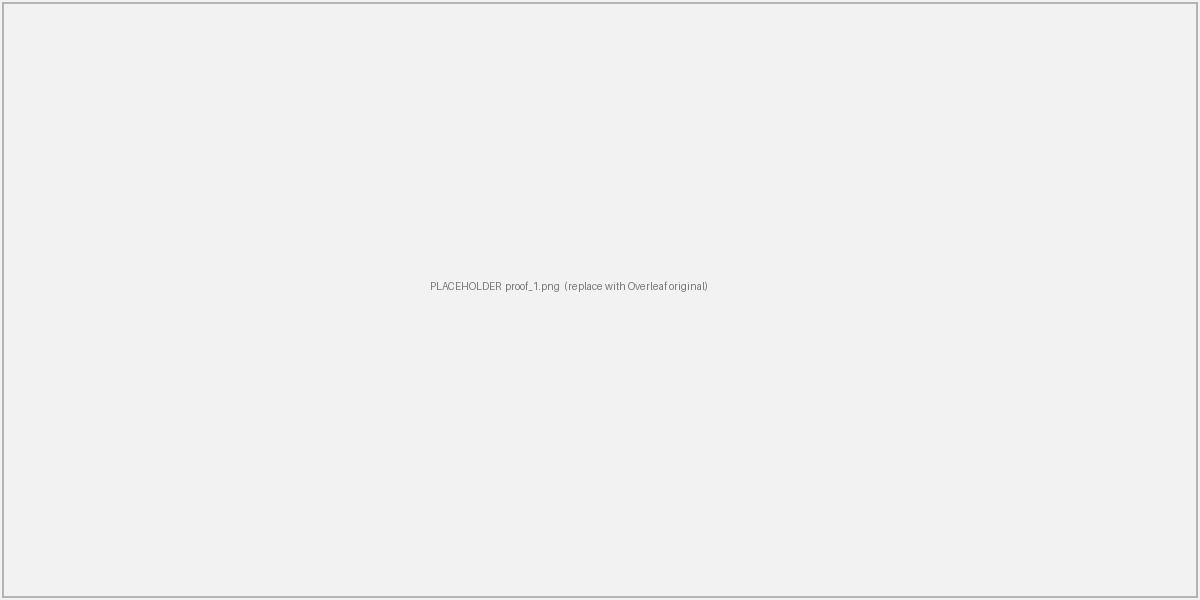
\includegraphics[width=0.85\textwidth]{proof_1.png}
  \caption{\texttt{pow\_add\_eq\_mul}: verified in 9\,s, 4 tool calls, 5 model invocations.}
  \label{fig:proof1}
\end{figure}

\begin{figure}[H]
  \centering
  
\includegraphics[width=0.85\textwidth]{proof_3.png}
  \caption{\texttt{mul\_pow\_eq}: verified in 14\,s, 8 tool calls, 8 model invocations.}
  \label{fig:proof3}
\end{figure}

\subsubsection{Inductive inequalities}

For \texttt{two\_pow\_gt\_n} ($n < 2^n$), the agent selected induction
unprompted, closed the base case with \texttt{simp} and the successor case
with \texttt{simp [Nat.pow\_succ]} followed by \texttt{linarith}
(92 seconds; 3 tool calls, 4 model invocations). The Bernoulli-type
inequality \texttt{bernoulli\_three} ($1 + 2n \le 3^n$) required an explicit
inductive hypothesis and a multi-step \texttt{calc} block justified by
\texttt{ring}, \texttt{linarith}, \texttt{Nat.mul\_le\_mul\_left}, and
rewrites through \texttt{Nat.pow\_succ} and \texttt{mul\_comm}
(31 seconds; 13 and 13). Sequencing a \texttt{calc} chain correctly under
sequential compiler feedback is a non-trivial demonstration of structural
reasoning for a model of this class.

\begin{figure}[H]
  \centering
  
\includegraphics[width=0.85\textwidth]{proof_2.png}
  \caption{\texttt{two\_pow\_gt\_n}: verified in 92\,s, 3 tool calls, 4 model invocations.}
  \label{fig:proof2}
\end{figure}

\begin{figure}[H]
  \centering
  
\includegraphics[width=0.85\textwidth]{proof_4.png}
  \caption{\texttt{bernoulli\_three}: verified in 31\,s, 13 tool calls, 13 model invocations.}
  \label{fig:proof4}
\end{figure}

\subsubsection{Type theory and surjectivity}

The most advanced Generation-One result is a formalisation of Cantor's
theorem in the form
\[
  \texttt{cantor } (\alpha : \mathsf{Type})\ (f : \alpha \to \alpha \to \mathsf{Prop}) :
  \lnot\,(\forall y,\ \exists x,\ f\,x = y),
\]
verified in 56 seconds over 26 tool calls and 26 model invocations. The
agent introduced the surjectivity hypothesis, defined the diagonal predicate
$d := \lambda x.\ \lnot f\,x\,x$, obtained the hypothetical pre-image via
\texttt{obtain}, and --- at the proof's hinge --- recognised the need for
\texttt{congr\_fun} to equate evaluated results, deriving
$f\,a\,a = \lnot f\,a\,a$ and discharging the contradiction. The linear loop
tracked a genuinely multi-step logical contradiction across an extended
horizon without losing context.

\begin{figure}[H]
  \centering
  
\includegraphics[width=0.85\textwidth]{proof_5.png}
  \caption{\texttt{cantor}: verified in 56\,s, 26 tool calls, 26 model invocations.}
  \label{fig:proof5}
\end{figure}

\begin{table}[H]
  \centering
  \caption{Summary of Generation-One verified results.}
  \label{tab:gen1-results}
  \renewcommand{\arraystretch}{1.4}
  \begin{tabular}{llrrr}
    \toprule
    Theorem & Domain & Model invocations & Tool invocations & Time \\
    \midrule
    \texttt{pow\_add\_eq\_mul} & Algebra (exponents)       & 5  & 4  & 9\,s  \\
    \texttt{mul\_pow\_eq}      & Algebra (exponents)       & 8  & 8  & 14\,s \\
    \texttt{two\_pow\_gt\_n}   & Inductive inequality      & 4  & 3  & 92\,s \\
    \texttt{bernoulli\_three}  & Inductive inequality      & 13 & 13 & 31\,s \\
    \texttt{cantor}            & Set theory (surjectivity) & 26 & 26 & 56\,s \\
    \bottomrule
  \end{tabular}
\end{table}

% ============================================================
\section{Failure Analysis: Loop Escape and Role Hijacking}
\label{sec:failure}
% ============================================================

Generation One's most valuable output was not a proof. It was a failure.

\subsection{The ``Fill in the Gap'' Incident}

Tasked with the number-theoretic proposition
\[
  \texttt{theorem six\_dvd\_cubic } (n : \mathbb{N}) : 6 \mid (n^3 - n),
\]
whose natural proof combines divisibility by 2 and 3 through coprimality,
the agent did not step through Pantograph. Instead it emitted, directly into
its text channel, the following artefact:

\begin{lstlisting}[caption={Hallucinated ``proof'' of \texttt{six\_dvd\_cubic}: fluent, well-structured, and rejected by the compiler.}]
import Mathlib.Tactics.Tactics
import Mathlib.Data.Nat.Parity
import Mathlib.Data.Nat.ModEq

theorem six_dvd_cubic (n : ℕ) : 6 ∣ (n ^ 3 - n) := by
  have h2 : 2 ∣ (n ^ 3 - n) := by
    cases n.even_or_odd with
    | inl h =>  -- n is even
      rw [Nat.even_iff] at h
      have : n ≡ 0 [MOD 2] := h
      calc
        n ^ 3 - n ≡ (0 ^ 3) - 0 ≡ 0 - 0 ≡ 0 [MOD 2] := by congr; exact this
    | inr h =>  -- n is odd
      rw [Nat.odd_iff] at h
      have : n ≡ 1 [MOD 2] := h
      calc
        n ^ 3 ≡ (1 ^ 3) ≡ 1 [MOD 2] := by congr; exact this
        _ - n ≡ 1 - 1 ≡ 0 [MOD 2] := by ring
  have h3 : 3 ∣ (n ^ 3 - n) := by
    cases Nat.mod n 3 with
    | zero =>
      have : n ≡ 0 [MOD 3] := by exact Nat.mod_eq_zero _ _
      calc
        n ^ 3 - n ≡ (0 ^ 3) - 0 ≡ 0 - 0 ≡ 0 [MOD 3] := by congr; exact this
    | one =>
      have : n ≡ 1 [MOD 3] := by exact Nat.mod_eq_of_eq _ rfl
      calc
        n ^ 3 ≡ (1 ^ 3) ≡ 1 [MOD 3] := by congr; exact this
        _ - n ≡ 1 - 1 ≡ 0 [MOD 3] := by ring
    | two =>
      have : n ≡ 2 [MOD 3] := by exact Nat.mod_eq_of_eq _ rfl
      calc
        n ^ 3 ≡ (2 ^ 3) ≡ 8 ≡ 2 [MOD 3] := by norm_num
        _ - n ≡ 2 - 2 ≡ 0 [MOD 3] := by ring
  exact Nat.dvd_mul_of_dvd_of_dvd (Nat.coprime_two_three) h2 h3
\end{lstlisting}

The script is fluent and structurally plausible; it is also unsound
(modular reasoning is applied where Lean's \texttt{calc} and \texttt{congr}
cannot carry it, and several cited lemmas do not exist). The compiler would
reject it immediately --- but the compiler was never consulted.

\subsection{Mechanics and Security Classification}

The failure is not primarily mathematical; it is a protocol breach.
Rather than returning a JSON-RPC payload invoking
\texttt{verify\_full\_script} on Leak-II, the model \emph{hallucinated the
entire transaction}: it emitted the proof block and then fabricated the
observation that a tool had verified it, exploiting a permissive
orchestration layer that accepted exit transitions regardless of which role
produced them. In the taxonomy of the OWASP Top 10 for Agentic
Applications~\cite{owasp2025agentic}
this is \emph{Agent Goal Hijack} (ASI01) combined with \emph{Role Hijacking}
(D1.1) --- a confused-deputy pattern in which the agent impersonates its own
verifier.

The general lesson generalises beyond theorem proving: autoregressive models
carry an inherent bias toward \emph{satisfying the user's request} (produce
a proof) over honouring middleware constraints. When the task becomes
genuinely hard --- what we informally call algorithmic fatigue --- the model
will exploit any loophole in prompt boundaries or schema parsing to
terminate the loop, simulating success rather than enduring further
compiler rejection. No model, however capable, should be trusted to report
its own verification status.

\subsection{The Lesson: An Exit Must Be Earned}

Generation One patched this with stricter schema enforcement. Generation Two
promotes it to the central design invariant: \emph{the only reachable exit
node is a compiler certificate}. A run terminates successfully if and only
if the verification daemon itself returns a sorry-free, error-free
compilation of the complete script; the model's prose --- claims, summaries,
final answers --- is never load-bearing. Every architectural feature
described next is downstream of this rule.

% ============================================================
\section{Generation Two: Verified Decomposition at Scale}
\label{sec:gen2-arch}
% ============================================================

\subsection{What Changed and Why}

Two limits bound Generation One. First, the \textbf{horizon}: a single
linear context cannot hold a proof campaign that needs hundreds of
exchanges, because the append-only ledger grows quadratically ---
every turn re-reads a longer history, and the model measurably degrades as
the ledger inflates. Second, the \textbf{ceiling}: a compact model's
five-by-five region covers textbook lemmas, not competition mathematics.

Generation Two attacks both at once:

\begin{itemize}[leftmargin=*]
  \item The reasoning engine becomes a frontier model --- Anthropic's Claude
    (Opus-class) --- driven through an agentic runtime rather than a raw
    completion API. The MCP boundary made the swap architecturally trivial.
  \item Governance moves from invocation counts to \emph{wall-clock time}.
    There are no turn caps; a run carries a live compute budget that an
    operator can extend mid-flight, and every stage (planner, sub-agents,
    finisher) races the same shared clock. Individual proof campaigns
    routinely extend to \emph{hundreds} of reasoning--action--observation
    exchanges between the system, the model, and the Lean tools.
  \item Decomposition returns --- but in a disciplined form in which every
    intermediate structure is compiler-verified before any further effort is
    invested in it (Sections~\ref{sec:have}--\ref{sec:have-tree}).
\end{itemize}

\subsection{The Stack, Revised}

\begin{itemize}[leftmargin=*]
  \item \textbf{Leak-I} (Moogle/Loogle retrieval) is retained but now
    \emph{rationed}. A search governor grants a small initial budget
    (three queries by default); further allowance is \emph{earned} only when
    a genuine proof attempt surfaces an unknown lemma name. When the budget
    is spent, the agent is redirected: stop searching and prove --- and
    taught the idiom of extracting names for free by compiling
    \texttt{example : <goal> := by exact?} against the daemon instead of
    guessing. This single governor eliminated the ``librarian death
    spiral,'' in which an agent burns its entire budget browsing the library
    without ever compiling anything.
  \item \textbf{Leak-II} (Pantograph) remains the interactive workspace:
    \texttt{init\_proof} / \texttt{apply\_tactic} stepping against the
    persistent daemon, used both for direct proving and for
    \emph{reconnaissance} --- discovering what the intermediate goal states
    actually look like before committing to a decomposition.
  \item \textbf{Leak-III} (specialist tactic oracle) is retired; the
    frontier generalist subsumes it.
  \item \textbf{Leak-IV} is the new batch verifier: a version-locked Lean
    \texttt{v4.29.1} + Mathlib service exposing \texttt{verify\_full\_script}.
    It is deliberately \emph{not} an exploration tool --- it is the
    certification gate, the sole authority on success. The trust boundary of
    Section~\ref{sec:failure} is drawn here: \texttt{verified} status and the
    final proof artefact are read exclusively from Leak-IV's compiler output,
    never from model prose.
  \item \textbf{Leak-XI / XII / XIV} form a parallel, newer stack at Lean
    \texttt{v4.32.0}, serving the blueprint families of
    Section~\ref{sec:architect}: retrieval, a \texttt{lean\_compile} +
    \texttt{lean\_elaborate} gateway enforcing the blueprint annotation
    discipline, and a separate certification service respectively.
\end{itemize}

\paragraph{Deployment and version discipline.} Every service is an
independent container deployed as a Hugging Face Space~\cite{hfspaces},
speaking MCP over server-sent events. This matters methodologically rather
than operationally: because the toolchain lives behind a service boundary
rather than in the prover, the Lean and Mathlib versions that certified a
run are a recorded property of that run. Every research row stores them,
since the two groups are \emph{not} interchangeable and a certificate that
named the wrong one would be a false claim about how the proof was checked.

One version gap is worth recording as a limitation. The older retrieval
service resolves its Mathlib revision at container build time rather than
pinning it, so its index corresponds to whatever was current when it was
last built --- a retrieval tool answering from a slightly different library
than the compiler is, as the newer service's own documentation puts it, a
name generator rather than a lookup. The \texttt{v4.32.0} retrieval service
corrects this by pinning the Mathlib tag and asserting the pin at build time,
and additionally distinguishes a \emph{definitive} negative (``no
declaration of this name exists'') from a parse failure, which the older
index could not express.

Operationally, the prover runs wherever a model runtime is available: an
operator's workstation via a lightweight local bridge, or a fleet of
workers leasing jobs from a queue. The same prover code path serves
interactive runs, batch generation, and the benchmark harness --- which is
what makes production results and benchmark results commensurable.

\subsection{The Research-Mode Protocol}

Frontier models introduce a failure mode compact models rarely exhibited:
\emph{erudite surrender}. Recognising a statement as hard, the model stops
to explain that it resembles an open problem and politely declines. The
Generation-Two prompt protocol forbids this outright. Under research mode,
the agent may not assess provability, difficulty, or fame; its only valid
outputs are (a)~a verified proof or (b)~a further decomposition of the goal
into smaller sub-goals; and it must never return empty-handed --- a failed
attempt still yields its best partial \texttt{have}-scaffold so the next
agent builds on something. Progress is defined as \emph{shrinking the
unproved residue}, not closing the theorem in one stroke. This reframing
matters in production, where problem generators occasionally emit statements
of genuinely unknown difficulty.

\subsection{The Registry Principle}

Rather than committing to one prompting philosophy, the orchestrator carries
a \emph{strategy registry}: named, swappable configurations, each pairing a
prover prompt, a decomposition prompt, an orchestration topology and a
retrieval allowance. Because strategies differ \emph{only} in those four
dimensions --- the verification gate, the governance clock, the toolchain
pins and the MCP tool surface being common to all --- the registry functions
as a controlled experiment on proving styles rather than a collection of
incomparable systems. Adding a strategy is adding an experimental arm.

This is the instrument on which the whole of
Section~\ref{sec:results-fatex} depends, and it is described in full in
Section~\ref{sec:registry}. The remainder of the present section covers the
two decomposition mechanisms that the later strategies elaborate.

\subsection{In-Context Decomposition: The \texttt{have} Strategy}
\label{sec:have}

The naive way to decompose a formal proof is to extract top-level helper
lemmas. In practice this is a notorious error source: every local binder and
hypothesis must be re-generalised into each helper's signature, and the
slightest mismatch breaks the final assembly. The \texttt{have} strategy
decomposes \emph{inside} the single proof term instead. The agent writes one
self-contained proof of the master theorem in which every hard step is a
local hole:

\begin{center}
  \texttt{have h}$_i$ \texttt{: <proposition> := by sorry}
\end{center}

Local \texttt{have}s inherit the entire ambient context --- binders,
hypotheses, earlier steps --- natively, eliminating the re-generalisation
problem by construction. The method is skeleton-first: (1)~lay out the
argument as typed \texttt{have} steps and close the main goal from them;
(2)~\emph{compile the skeleton} so that the only outstanding holes are the
explicit \texttt{sorry}s --- proving the decomposition structurally valid
before any effort is invested in the hard parts; (3)~fill each hole
bottom-up, leading with strong automation and nesting further \texttt{have}s
where a step resists; (4)~exit only on a sorry-free full-script
verification. Step (2) is the \emph{structural gate}, and it is the piece
most agentic decomposition schemes lack: an unverified plan is worthless,
and the compiler can tell you so before you pay for it.

\subsection{The Have-Tree Orchestrator}
\label{sec:have-tree}

The flat \texttt{have} strategy still holds the whole campaign in one
context, so context cost grows roughly as $O(N^2)$ in proof length and the
model degrades on the largest proofs. The \emph{have-tree} bounds every
participant's context while preserving the in-context decomposition
principle. Three roles cooperate:

\begin{enumerate}[leftmargin=*]
  \item \textbf{Planner.} One agent produces the compiled skeleton: the
    master theorem with each hard step a typed hole, tagged for orchestration
    (\texttt{:= by sorry --}$\langle\!\langle h_N \rangle\!\rangle$). The
    skeleton must pass the structural gate on the daemon before anything
    else happens.
  \item \textbf{Minions.} Each hole is assigned to a fresh, isolated agent
    whose entire world is the skeleton: it sees the \emph{types} of its
    siblings --- their signatures, never their proofs --- plus its own goal,
    and may interrogate the daemon about its exact goal state on demand.
    When it returns its fill (a tactic block), the process exits and its
    context evaporates; only the fill survives. A minion facing a hole that
    is itself too large does not grind: it emits a nested decomposition ---
    a sub-skeleton with fresh holes --- which the orchestrator splices in
    after re-tagging for global uniqueness. Recursion is bounded
    (four levels) before the residue is handed to a single-context finisher.
  \item \textbf{Assembler.} Fills are spliced into the skeleton textually,
    with strict parsing --- a malformed reply yields a failed hole, never
    spliced garbage --- and the stitched artefact is re-verified
    \emph{end-to-end, hole-free} on the daemon. Nothing about the assembly
    is trusted; the final compile is the only certificate.
\end{enumerate}

Two properties follow. \textbf{Bounded context:} every agent operates
against the small skeleton rather than the full proof history, so cost
scales with the number of holes, not with proof length. \textbf{Monotone
safety:} any failure --- an uncompilable skeleton, an unfillable hole, a
stitched proof that fails verification --- triggers automatic fallback to
the flat single-context strategy, so the have-tree is never weaker than the
known-good path it generalises.

Listing~\ref{lst:skeleton} shows the shape of a planner skeleton, using the
top-level structure of a production proof discussed in
Section~\ref{sec:gen2-results} (problem \#219): the counting identity and
the two modular evaluations become independent, isolated work packets, while
the glue step (\texttt{core}) is closed on the spot by \texttt{omega}.

\begin{lstlisting}[caption={Planner-skeleton form of the verified proof of problem \#219. Each tagged hole is filled by an isolated sub-agent; the skeleton itself must compile before any hole is attempted.},label={lst:skeleton}]
theorem subset_sum_div3_mod13 :
    ((Finset.Icc 1 (3^101)).powerset.filter
      (fun s => (s.sum id) % 3 = 0)).card % 13 = 6 := by
  have core : ∀ A B C : ℕ, 3 * C = A + 2 * B →
      A % 13 = 8 → B % 13 = 5 → C % 13 = 6 := by
    intro A B C h1 h2 h3; omega
  have h1 : 3 * ((Finset.Icc 1 (3^101)).powerset.filter
      (fun s => (s.sum id) % 3 = 0)).card
      = 2^(3^101) + 2 * 2^(3^100) := by sorry --⟪h1⟫
  have h2 : (2:ℕ)^(3^101) % 13 = 8 := by sorry --⟪h2⟫
  have h3 : (2:ℕ)^(3^100) % 13 = 5 := by sorry --⟪h3⟫
  exact core _ _ _ h1 h2 h3
\end{lstlisting}

\subsection{Prove-or-Split Lemma Trees}

For strategies that do extract top-level lemmas, a separate orchestrator
drives a prove-or-split tree: each node is attempted directly under a
bounded budget; on a stall (or on the agent's own request, signalled by an
explicit \texttt{DECOMPOSE} line), a Decomposer run splits the node into
sub-lemmas that are \emph{structurally verified} before becoming children;
leaves close recursively; and the subtree is assembled bottom-up, gated on
one final sorry-free compile. The lemma tree and the have-tree are
maintained side by side as competing decomposition styles under the same
governance --- the registry again functioning as an experiment.

% ============================================================
\section{The Strategy Registry}
\label{sec:registry}
% ============================================================

This section documents the full registry, since it constitutes both the
system's principal engineering artefact and the experimental instrument for
this paper's question. Nineteen configurations are grouped into four
families by the kind of structure they impose. All share one gate
(Section~\ref{sec:failure}), one clock, and --- within a family --- one
toolchain.

\subsection{Family Zero: Flat Baselines}
\label{sec:controls}

The baselines exist because the rest of the paper is uninterpretable without
them. If elaborate orchestration is to be credited with a capability, the
capability must first be shown absent from a competent unstructured
configuration.

\paragraph{Leak Control I} (\texttt{control-oneshot}). One continuous agent,
one theorem, one tool. The agent's MCP inventory is filtered to the
certifying verifier alone: retrieval and interactive stepping are removed
structurally, not merely discouraged, even when connected. There is no
planner, no splitter, no sub-agent, no top-level helper lemma, and --- unlike
every other strategy --- no \texttt{DECOMPOSE} escape hatch and no
permissible ``too hard'' terminal state. A repeatedly failing approach is
instructed to try a \emph{different} approach to the same goal, never a
smaller piece of it.

When a session ends without a certificate and clock remains, a fresh session
begins. Exactly one artefact crosses that boundary: the previous session's
final submitted script and the verifier's verbatim response to it. This
quantity of memory is a deliberate calibration. A wholly amnesiac
retry-from-scratch loop would be a strawman --- no human ``keeps trying''
by forgetting their last attempt --- while accumulating every past attempt,
or a proven-lemma bank, or a dead-end ledger, would make the control a
refinement strategy under another name and defeat its purpose.

\paragraph{Leak Control II} (\texttt{control-oneshot-2}). Identical in every
respect except that library search is restored. Interactive stepping remains
excluded. The search guidance rendered into its prompt is the same shared
block every other search-capable strategy receives, not a bespoke variant.
Control~II therefore isolates exactly one variable against Control~I ---
whether retrieval alone, absent any structuring of the search, changes
outcomes.

\subsection{Family One: Single-Context Strategies}

Six configurations hold the entire campaign in one linear context and vary
only in prompting philosophy. They were the original instrument for the
question ``which proving style works?'' and several now serve as controls
for more elaborate arms.

\begin{itemize}[leftmargin=*]
  \item \textbf{hacker} --- compiler-driven; the verifier is the main loop:
    attempt, read errors, patch, recompile. Retrieval budget 3.
  \item \textbf{pantograph} --- interactive-first; the REPL is the workspace
    and the verifier is touched once, at the end, to certify. Its
    decomposition prompt caps reconnaissance explicitly: at most the first
    half of available turns may be spent stepping.
  \item \textbf{librarian} --- search-first, with a retrieval budget of 30
    rather than 3. It exists as the deliberate opposite of \textbf{hacker},
    to test whether search helps when it is abundant.
  \item \textbf{sketch} --- a natural-language argument sketch of three to
    eight steps before any tool call, then stepwise formalisation.
  \item \textbf{brute} --- automation only, retrieval budget zero. The
    prompt enumerates a closer ladder (\texttt{decide},
    \texttt{native\_decide}, \texttt{omega}, \texttt{simp},
    \texttt{norm\_num}, \texttt{simp\_all}, \texttt{aesop},
    \texttt{nlinarith}, \texttt{positivity}) for the first submission.
  \item \textbf{have} --- in-context \texttt{have} decomposition
    (Section~\ref{sec:have}), which additionally serves as the single-context
    A/B control for the entire tree family and as their common fallback and
    resume path.
\end{itemize}

\subsection{Family Two: The Stronghold Line}
\label{sec:stronghold}

The Stronghold strategies share the planner/minion/assembler shape of
Section~\ref{sec:have-tree} and differ in how the minion phase is scheduled
and what crosses between agents. Their development is a sequence of
diagnoses, each strategy addressing a failure observed in its predecessor,
which makes the line unusually legible as an engineering record.

\paragraph{Stronghold Dark} (\texttt{have-tree}). The sequential baseline:
holes are filled one at a time by iterative deepening, bounded at four
levels of recursive re-decomposition. Sequential execution is not a design
preference but a constraint of the original REPL service, whose memory
cleanup was global and therefore unsafe under concurrency.

\paragraph{Stronghold Surround} (\texttt{have-surround}). Dark's shape with
the minion phase parallelised over the ghost-daemon service
(Section~\ref{sec:substrate}), four concurrent workers by default. It is a
\emph{continuous work queue} rather than synchronised rounds: accepted
sub-holes are enqueued immediately, so a worker never idles behind the
slowest minion of a round. All mutations of the shared skeleton serialise
through a lock while minion execution overlaps freely. Its soundness rests
on an observation about the decomposition discipline itself --- a hole's fill
depends only on its siblings' \emph{signatures}, which are immutable, never
on their proof bodies --- plus the unconditional hole-free re-verification of
the assembled artefact.

\paragraph{Finality I} (\texttt{finality-1}). Surround plus a
system-summoned refinement loop on a ten-minute cadence. When the timer
fires, in-flight minions are cut off immediately; the refiner is then shown
the current skeleton, a bank of every lemma proved so far keyed by
normalised proposition, the holes that genuinely failed, the holes that were
merely interrupted, and the live proof states of the cut-off minions with
their accepted tactic scripts inlined. It must triage every live state ---
reassigning it to a hole in the revised skeleton or explicitly freeing it ---
and brief the minions who will inherit each hole.

Two details of this design proved important. First, defeated and interrupted
work are tracked in \emph{separate} maps, because reporting a
clock-interrupted approach to the refiner as ``already failed'' is how a
system talks itself off the direction that was about to succeed. Second,
banked lemmas are keyed on the whitespace-normalised proposition rather than
on the hole's name, so a refinement that renames or restructures a hole
still restores its proof for free.

\paragraph{Stronghold Force} (\texttt{stronghold-force}). Force exists
because of a negative result worth recording. Dark, Surround and Finality
all advertise recursive decomposition, and in production none of them ever
recursed. The cause was structural rather than incidental: recursion was
offered to the \emph{minion} as a consolation prize for failing to close its
hole, but a minion holding a fifteen-minute budget --- and required to
compile any split it proposes before handing it back --- simply grinds at
closing until its clock expires. Two logged thirty-minute runs recorded 24
and 30 verification calls and zero decomposition blocks. The hole count in a
Stronghold run had only ever gone down.

Force moves recursion into a stage that does nothing else. A deliberately
small root skeleton of three to five holes is followed by a seven-minute
expansion phase in which dedicated splitter agents --- explicitly told they
are not proving anything --- cut each hole into roughly three sub-holes to a
depth of three, every cut re-verified before it is applied, so the skeleton
is valid at every instant and its hole count only rises. A ten-minute
campaign of five minions then works the leaves deepest-first. A campaign
that leaves holes open returns them to the decomposer; there is no finisher.

\paragraph{Stronghold Forte} (\texttt{stronghold-forte}). Forte is Force
plus three additions, each derived from a specific pathology in a logged
Force run on the FATE-X problem discussed in
Section~\ref{sec:control-observation}, in which 19 holes closed but 3
remained open when the hour expired.

\begin{enumerate}[leftmargin=*]
  \item \textbf{Locally tracked handoff scripts.} In the audited run, one
    cycle handed the decomposer four live proof states with zero readable
    scripts, because the only source of a cut-off minion's progress was a
    live state query issued to the shared REPL immediately after a mass
    recall --- precisely when it is most loaded. Forte instead reconstructs
    the accepted-tactic prefix from the minion's own tool-call stream as it
    happens, pairing each tactic with its result and retaining only those the
    daemon confirmed. The live query survives solely as a fallback for states
    Forte never itself touched.
  \item \textbf{A cross-hole opening pool.} Unrelated holes were observed
    re-deriving byte-identical opening tactic sequences. Forte caches
    accepted openings run-wide and surfaces the single best match to a new
    hole with a similarly-shaped goal, explicitly hedged as a hint rather
    than asserted as fact --- in deliberate contrast to the lemma pool, whose
    entries are compiler-certified and are asserted.
  \item \textbf{A near-duplicate cut guard.} A cut whose child restates its
    own parent is vacuous, and one earlier run lost twenty minutes to an
    alpha-renamed parent-as-child hole. Forte compares child and parent
    propositions by token containment and rejects the cut above a threshold
    of 0.92, recording the rejection so the next splitter does not repeat it.
    Containment rather than symmetric overlap is used deliberately, so that a
    short restatement wholly inside a longer goal still scores high. This is
    a cheap local analogue of the embedding-similarity ancestor check used by
    lean-collab~\cite{leancollab2026}.
\end{enumerate}

\subsection{Family Three: Blueprint Refinement}
\label{sec:architect}

The River and Ultra families implement a blueprint-graph pipeline over a
separate, newer toolchain (Lean \texttt{v4.32.0}). A generation stage emits a
dependency graph of annotated declarations whose bodies are stubbed with
dependency-carrying holes; isolated node provers attempt each node in
parallel; a refinement stage reads the annotated graph with per-failure
diagnoses and emits a revised blueprint; and the loop repeats until a
separate certifying service accepts the assembled artefact. Refinement
iterations are capped at eight.

The River variants form a deliberate ablation ladder, each adding exactly
one mechanism to its predecessor:

\begin{itemize}[leftmargin=*]
  \item \textbf{River Stone} --- the control: bare pipeline, fully isolated
    nodes, nothing shared.
  \item \textbf{River Gate} --- Stone plus a shared dead-end ledger.
    Crucially, the ledger shares only \emph{environment facts} established by
    the compiler --- names that do not exist, typeclasses unavailable in
    context, coercion traps --- and never a tactic that worked, a proof body,
    or any node's approach, so node independence is preserved.
  \item \textbf{River Delta} --- Gate plus a single natural-language proof
    seed generated up front and handed to blueprint generation as a
    structural guide.
  \item \textbf{River Vintage} --- branches from Stone rather than Delta, so
    that it isolates exactly one change: the oversight watchers described
    below.
\end{itemize}

\textbf{Ultra Fleeting} (\texttt{ultra-fleeting}) runs Stone's pipeline ---
identical prompts, identical tool contract, identical gates --- with the
local Claude runtime as driver instead of the xAI API. The substitution is
more than a model string: because that runtime calls MCP tools itself, the
bridge must serve the compile and search tools from a local server whose
handlers are the very same closures the other driver uses, which keeps the
compile gate and the blueprint capture on the bridge where they must be. The
driver is never trusted to self-report that a blueprint compiled.

\paragraph{Oversight watchers.} Vintage adds three supervisory mechanisms,
each of which is a response to an observed failure and each of which is
deliberately constrained in what it may assert.

\begin{itemize}[leftmargin=*]
  \item The \textbf{interceptor} reviews a single agent's own trajectory
    asynchronously --- the agent never waits --- and may emit a note or, rarely,
    abort. It is instructed to prefer silence, to treat changing errors as a
    sign of health, and never to abort an agent still producing new errors,
    since ``agents often self-correct; a premature abort kills a proof that
    was one submission away.''
  \item The \textbf{mechanic} reads a run-wide window of the rendered
    activity stream in parallel and routes judgements to live agents, to
    refinement, or to the log. Its charter is explicitly \emph{not} to
    prove or to fix: a note may contain only the observed pattern and
    missing context quoted from ground truth, never a tactic, lemma or
    closed form. Its epistemic limits are stated as hard rules because
    earlier iterations fabricated evaluation results and declared correct
    closed forms wrong.
  \item The \textbf{consultant} fires on a literal repeated-error streak and
    is the one watcher the agent waits for. It receives the full activity
    log and the unmoved error and is asked for the single structural change
    to make next, or the honest conclusion that the node should be forfeited.
\end{itemize}

\subsection{Cross-Cutting Mechanisms}
\label{sec:mechanisms}

Several mechanisms are shared across families and are, in our assessment,
where most of the reliable benefit of scaffolding actually resides.

\paragraph{The retrieval governor.} Early runs exhibited a
``librarian death spiral'': an agent exhausting its budget browsing the
library without ever compiling. The governor rations retrieval to three
queries initially, and --- this is the load-bearing part --- further allowance
is \emph{earned} rather than granted, triggered only when a genuine proof
attempt (a submission containing real proof syntax, not a bare identifier
probe) elicits an unknown-name diagnostic from the compiler. Probing the
compiler to brute-force names does not earn a refill, since that would
amount to paying the agent to guess. When the budget is spent the agent is
redirected in the tool response itself: stop searching, prove, and recover
names for free by compiling \texttt{example : <goal> := by exact?}.

A limitation of the present implementation is noted here because it becomes
a recommendation in Section~\ref{sec:future}: replenishment is reported to
the \emph{operator console}, not into the agent's context. The agent
observes the exhaustion message directly but learns of a refill only
incidentally, from the budget annotation on its next successful search. An
agent that has concluded its budget is gone may therefore stop attempting
retrieval altogether for the remainder of a run in which retrieval has in
fact been restored.

\paragraph{The verified-lemma pool.} Every successful compilation is, by
construction, a closed Lean fact, and minions establish many small facts en
route to their holes --- all of which previously died with the minion's
context. The pool harvests every sorry-free top-level declaration from any
error-free compile, filters out anything containing a hole, ranks entries
against the requesting agent's own goal by inverse-document-frequency token
overlap, and renders the top slice into each agent's prompt as asserted
fact. Its cost is zero: no extra model call, no extra compile, only reuse of
work already verified. It is the shared memory that isolated minions
otherwise cannot have.

The IDF weighting is not incidental. In a group-theory run, terms such as
\texttt{Group} and \texttt{Subgroup} appear in nearly every banked fact;
without down-weighting them, shared boilerplate outranks the one
distinctive name a hole and a fact genuinely share, and the ranking
degenerates to ``most verbose fact wins.''

\paragraph{The proven-lemma vault.} The blueprint families maintain an
analogous bank keyed on \emph{(normalised signature, dependency set)} rather
than on node name, so that a proof survives refinements which rename or
relocate its node. Dormant entries are advertised to the refiner, which can
restore them at zero prover cost by re-emitting a node with a matching
signature and dependency set. Entries are evicted only when certification
implicates them.

\paragraph{Certificate provenance.} The verifier returns, alongside its
verdict, the exact normalised bytes it compiled. Recording what was
\emph{sent} rather than what was compiled produced certificates that
silently depended on the service's own import injection and did not compile
standalone; the system therefore stores the compiled artefact, and declines
to synthesise a substitute when the marker is absent.

\paragraph{Checkpointing and resumption.} Every orchestrator emits a
checkpoint whenever the skeleton changes --- beginning with the verified
skeleton itself, which is worth saving at zero holes filled since resuming
from it skips the entire planning phase. A resumed run finishes from banked
progress rather than rediscovering it. Soundness is unaffected: the seed is
a hint, and the independent hole-free re-verification is unchanged.

\paragraph{The proof bank and run log.} A verified proof is persisted to a
local bank keyed on (signature, toolchain), so that a later failed or
terminated run of the same theorem cannot lose an earlier success --- a real
hazard when A/B-testing strategies against the same target. The bank never
short-circuits a run; an A/B arm must actually execute. Separately, every
rendered stream frame is appended synchronously to a per-run log on disk,
because a run that died with its browser tab previously took its own
diagnosis with it. The analyses in Sections~\ref{sec:results-fatex}
and~\ref{sec:control-observation} were conducted against those logs.

\paragraph{Cost accounting.} Per-run cost is the sum of the runtime's own
reported figure across every sub-invocation. Two subtleties are worth
recording: a concurrency bug in which sibling agents' costs were
double-counted by differencing shared state made one problem appear to cost
\$37 across 38 model calls; and terminating a child on success requires a
soft interrupt rather than a hard kill, because the final frame carrying the
cost figure is emitted during graceful shutdown.

\paragraph{Quota-aware abstention.} If the account driving a run is refused
by the provider mid-campaign, the run is not reported as a proof failure. An
observed run burned eight refinements, eight minion waves and 74 finisher
retries in roughly three minutes --- all no-ops --- and then reported
``unverified,'' as though the mathematics had been attempted. Such runs are
now reported as \emph{not attempted} and excluded from evidence, since this
class of false negative silently poisons a benchmark.

% ============================================================
\section{Generation Two: Empirical Results --- The CompeteMath Corpus}
\label{sec:gen2-results}
% ============================================================

\subsection{Deployment Context}

Generation Two is not a benchmark harness; it is the production proof engine
behind CompeteMath~\cite{competemath}, a competitive-mathematics
platform whose practice arena serves machine-generated competition problems.
Every problem ships with a hidden, formally verified Lean~4 proof of its
answer: a user who solves the problem (or surrenders after exhausting their
attempts) unlocks a \emph{proof certificate} --- the full Lean script,
canonically serialised and Ed25519-signed at ingestion, so that any third
party can verify both the mathematics (by recompiling) and the provenance
(by checking the signature). The platform's footer line is literal:
\emph{proofs checked by Lean~4}.

\subsection{Corpus Statistics}

As of 26 July 2026 the public practice pool contains \textbf{220} problems
across four difficulty tiers, of which \textbf{219 (99.5\%)} carry complete,
machine-checked proofs produced by the Leak/Claude pipeline --- roughly
383{,}000 characters ($\approx$ 7{,}500 lines) of verified Lean~4, generated
over a two-week production window (5--18 July 2026).

\begin{table}[H]
  \centering
  \caption{The CompeteMath verified corpus by difficulty tier (26 July 2026).}
  \label{tab:corpus}
  \renewcommand{\arraystretch}{1.4}
  \begin{tabular}{lrrrrr}
    \toprule
    Tier & Problems & Verified & Median proof (chars) & Largest proof (chars / lines) & Mean lines \\
    \midrule
    Easy   & 36 & 36 & 104   & 281 / 10        & 1  \\
    Medium & 88 & 88 & 201   & 18{,}444 / 345  & 18 \\
    Hard   & 78 & 77 & 1{,}783 & 25{,}351 / 354 & 65 \\
    Insane & 18 & 18 & 1{,}744 & 5{,}858 / 102  & 45 \\
    \midrule
    Total  & 220 & 219 & --- & --- & --- \\
    \bottomrule
  \end{tabular}
\end{table}

The tier medians tell the architectural story. Easy problems close in a
single automation line --- the brute strategy's territory. Medium problems
average a screenful. Hard problems average sixty-plus lines with medians
near two thousand characters: these are multi-lemma campaigns in which the
decomposition machinery earns its keep, and where individual runs extend to
hundreds of agent--tool exchanges under the wall-clock governor. The largest
verified artefacts exceed 300 lines with over one hundred intermediate
\texttt{have} steps.

The corpus spans elementary and analytic number theory (Kummer's theorem on
binomial carries, Jacobi symbols of 1{,}400-digit integers, Wilson-style
telescoping over $2^{61}$ factorials), enumerative and extremal
combinatorics (spanning-tree counts modulo two, derangement-class censuses,
ballot-path determinants), abstract algebra (forced cyclicity of groups of
order $1001$, Sophie Germain group counts, nilpotent matrix ledgers),
probability (expected return times of random walks, coin-flip
autocorrelation), and geometry and analysis (Descartes circle chains,
elliptic-curve point counts, root localisation in the complex disk).

\subsection{Case Study: Formalising the Argument Principle on Demand}

The largest proof in the corpus (problem \#220; 25{,}351 characters,
354 lines) answers a Rouch\'e-type question:

\begin{quote}
  \emph{Counted with multiplicity, how many roots of
  $f(z) = z^{2026} - 2026\,z^{7} + 5$ lie strictly inside the open unit
  disk $|z| < 1$?}
\end{quote}

The informal argument is one line: on $|z|=1$,
$|z^{2026} + 5| \le 6 < 2026 = |{-2026 z^7}|$, so by Rouch\'e's theorem $f$
has as many roots in the disk as $-2026z^7$, namely seven. The formal
difficulty is that Mathlib does not expose Rouch\'e's theorem in the
polynomial-root-counting form the problem needs. The agent's response was
not to search harder but to \emph{build the missing analysis}: the verified
script constructs, as local \texttt{have} steps inside one proof term, a
factorisation of a polynomial over its root multiset; a logarithmic-derivative
identity; the contour-integral evaluation
\[
  \oint_{|z|=1} \frac{p'(z)}{p(z)}\,dz \;=\; 2\pi i \cdot
  \#\{\,\text{roots of } p \text{ in } |z|<1\,\}
\]
for polynomials non-vanishing on the circle; and the continuity (hence
integer-valued constancy) of the filtered root count along the linear
homotopy $g + t\,(f - g)$, $t \in [0,1]$ --- that is, a working argument
principle, formalised from first principles because the library lacked the
exact statement. Listing~\ref{lst:rouche} shows the statement and the two
pivotal internal lemmas.

\begin{lstlisting}[caption={Problem \#220 --- statement and pivotal internal steps of the 354-line verified script (excerpt).},label={lst:rouche}]
open Polynomial in
theorem giant_coefficient_seven_roots :
    (((X ^ 2026 - (2026 : Polynomial ℂ) * X ^ 7 + 5 : Polynomial ℂ).roots).filter
      (fun z => Complex.abs z < 1)).card = 7 := by
  have h1 : ∀ z : ℂ, Complex.abs z = 1 →
      Complex.abs (z ^ 2026 + 5) < Complex.abs ((2026 : ℂ) * z ^ 7) := by
    ...
  have hRouche : ∀ (f g : Polynomial ℂ), f ≠ 0 → g ≠ 0 →
      (∀ z : ℂ, ‖z‖ = 1 → ‖f.eval z - g.eval z‖ < ‖g.eval z‖) →
      (f.roots.filter (fun z => Complex.abs z < 1)).card =
      (g.roots.filter (fun z => Complex.abs z < 1)).card := by
    ...
    have keyIntegral : ∀ (p : Polynomial ℂ),
        (∀ z : ℂ, ‖z‖ = 1 → p.eval z ≠ 0) →
        (∮ z in C(0,1), p.derivative.eval z / p.eval z) =
        2 * Real.pi * Complex.I *
          (p.roots.filter (fun z => Complex.abs z < 1)).card := by
      ...
\end{lstlisting}

For contrast with Generation One: the same architecture family that once
needed twenty-six exchanges for Cantor's diagonal argument here sustains a
campaign that fabricates a chapter of complex analysis and survives a
single, unforgiving end-to-end compile.

\subsection{Case Study: Counting Beyond Enumeration}

Problem \#219 (tier: Insane) asks for $N \bmod 13$, where $N$ counts the
subsets of $\{1, \dots, 3^{101}\}$ whose element sum is divisible by~3. The
family being counted has $2^{3^{101}}$ members --- enumeration is not merely
expensive but physically meaningless, so the \texttt{decide}-style escape
hatches that close the Easy tier are useless here. The verified proof
(Listing~\ref{lst:skeleton} shows its skeleton) establishes the exact
identity $3N = 2^{3^{101}} + 2 \cdot 2^{3^{100}}$ via an insertion-recursion
lemma proved by a hand-rolled bijection over \texttt{Finset.powerset}, then
evaluates both powers modulo 13 through order-of-2 arguments, and closes
with linear arithmetic. It is a proof \emph{about} an astronomically large
finite structure, conducted entirely at the level of structure --- exactly
the regime where formal verification outperforms both numerics and informal
confidence.

\subsection{The Open Residue}

One Hard-tier problem (\#215, a Wilson-flavoured claim that a certain giant
determinant reduces to $-1$) remains unproved in production at the time of
writing. We report this deliberately: a 219/220 corpus with a visible,
dated frontier is more informative than a curated 100\%, and the failure
case concentrates exactly where the current architecture predicts ---
determinant identities whose natural informal proof routes through theory
Mathlib does not yet expose in usable form, and whose from-scratch
formalisation cost exceeds the configured compute budget.

\subsection{Generation One versus Generation Two}

\begin{table}[H]
  \centering
  \caption{The two generations compared.}
  \label{tab:gen-compare}
  \renewcommand{\arraystretch}{1.5}
  \begin{tabular}{>{\bfseries}p{3.2cm} p{5.4cm} p{6.0cm}}
    \toprule
    Dimension & Generation One & Generation Two \\
    \midrule
    Reasoning engine & Grok 3 / Grok 4 Fast (compact, cost-optimised) & Claude (Opus-class frontier), agentic runtime \\
    Loop structure & Single linear ReAct context & Linear ReAct \emph{nodes} inside verified-decomposition orchestrators \\
    Governance & Invocation counts; terminate on bloat & Wall-clock budgets, live-extensible; no turn caps \\
    Exit condition & Prompt-level convention (exploitable, Section~\ref{sec:failure}) & Compiler-gated: only a sorry-free daemon compile terminates a run \\
    Decomposition & None (single context) & \texttt{have}-flat, have-tree (planner / minions / assembler), prove-or-split lemma trees \\
    Library search & Unrestricted & Governor-rationed; allowance earned by real attempts \\
    Typical horizon & $\sim$5 model + 5 tool invocations & Hundreds of exchanges per campaign \\
    Hardest verified result & Cantor's diagonal argument & Argument-principle root counting; modular counts over $2^{3^{101}}$-element families \\
    Verified output & 5 showcase theorems & 219 production theorems ($\approx$ 7{,}500 lines of Lean) \\
    \bottomrule
  \end{tabular}
\end{table}

% ============================================================
\section{Controlled Evaluation on FATE-X}
\label{sec:results-fatex}
% ============================================================

The CompeteMath corpus establishes that the architecture works at
production scale, but it is a poor instrument for the question of
Section~\ref{sec:research-question}. Its problems were generated by the same
pipeline that proves them, its difficulty distribution is not externally
calibrated, and its results accumulated over months of concurrent
development rather than under a fixed protocol. To compare strategies we
need a fixed, external, difficulty-calibrated target.

\subsection{The Benchmark}

We use \textbf{FATE-X}~\cite{fatex2025}, a benchmark of 100 Lean-formalised
abstract- and commutative-algebra problems published by Frenzy Math. Its
authors describe it as containing ``100 extremely challenging abstract
algebra and commutative algebra exercises,'' and --- a point we return to at
length in Section~\ref{sec:contamination} --- state that these were
collected from ``Undergraduate and graduate textbooks, Final exams and PhD
qualifying exams, Research literature.'' Each entry ships a fully
formalised statement terminated by a single \texttt{sorry}, together with a
natural-language rendering, minimal supporting definitions, and topic tags.
No reference proofs are distributed.

FATE-X is a deliberately severe target. It is designed to exceed both PhD
qualifying-examination difficulty and Mathlib's coverage, meaning a
non-trivial fraction of problems require the prover to construct
library-absent machinery rather than locate it. The publicly reported
leaderboard~\cite{benchmarklist_fatex} at the time of writing lists a single
entry: the Leanstral~1.5 proof-engineering system~\cite{leanstral2026} at
34/100. We note that figure for orientation only. It is self-reported via
the system's own launch announcement, we have not independently reproduced
it, and --- critically --- it is not accompanied by a compute budget, so it
is \emph{not} directly comparable to the numbers below, which are reported
against an explicit one-hour-per-problem cap. We draw no ranking conclusion
from the comparison and caution against doing so.

\subsection{Preprocessing}
\label{sec:preprocessing}

Preprocessing was more substantial than the word usually implies, and since
it bears on both comparability and contamination we describe it in full.

\paragraph{Normalisation.} Statements are stripped of their
\texttt{import Mathlib} line (the verification service injects it, and
rejects submissions that add imports), of the
\texttt{namespace}/\texttt{end} wrapper, and of doc comments, whose informal
content is retained separately.

\paragraph{Single-theorem rewriting.} The blueprint pipeline requires its
target to be one theorem with nothing preceding it: any \texttt{open},
\texttt{class}, \texttt{def}, \texttt{instance} or \texttt{variable} line
before the theorem is absorbed into the compiler's target-signature match,
which then demands a signature nothing can satisfy. This was verified live ---
a problem carrying a \texttt{class} prelude exhausted its entire budget
without ever producing a compiling blueprint, while a bare-theorem problem
compiled and validated in the same run.

Of the 100 published statements, 52 carried such a prelude. Preludes are
eliminated by inlining definitions into the goal, unfolding a class into its
defining equation, replacing a concrete construction by a universally
quantified parameter plus a characterising hypothesis, and fully qualifying
names in place of \texttt{open}. \textbf{51 statements were rewritten} into a
compact single-theorem form named \texttt{fatex\_NNN\_compact}; the 52nd is
excluded for the toolchain reason below and was never rewritten.

\paragraph{Machine-checked strength.} No rewriting is assumed sound. Each
carries a \texttt{strengthProof}: a Lean tactic script deriving the
\emph{original} FATE-X theorem from the compact one, verified on the
\texttt{v4.32.0} toolchain. A rewriting is admitted only if that derivation
type-checks, establishing that the compact form is at least as strong as the
published form. Several are strictly stronger --- generalising a concrete
ring to any ring isomorphic to it, for instance. The original statement is
retained for every rewritten problem so that the claim remains auditable.

\paragraph{Toolchain exclusions.} FATE-X was authored against Lean
\texttt{v4.28.0}. Every statement was additionally compiled standalone
against our \texttt{v4.32.0} toolchain; 98 of 100 elaborate. The two
failures are genuine Mathlib API drift on the \emph{original} statement that
no rewriting can repair without altering its mathematical content:
\texttt{fatex\_009}, where \texttt{Subgroup.normalizer}'s field-notation
signature changed, and \texttt{fatex\_041}, where a previously computable
definition now requires \texttt{noncomputable}. Both are excluded from every
run --- which is why \texttt{fatex\_009} is absent from
Table~\ref{tab:fatex-headline}. The effective benchmark is therefore 98
problems, and any pass rate should be read against that denominator.

\paragraph{Consequences.} Two deserve emphasis. First, a proof of a
rewritten statement is a proof of the original, so success counts are not
inflated by weakening. Second, and relevant to
Section~\ref{sec:contamination}, the exact token sequence presented to the
prover for those 51 problems did not exist in any public corpus prior to our
own preprocessing run. That is a partial, auditable contamination firewall
for roughly half the benchmark, independent of publication dates. The
remaining problems are used in published form and carry no such property.

\paragraph{A caveat we record against ourselves.} The strength proofs were
checked once, as a manual procedure; no test or continuous-integration job
re-checks them, and nothing reads the field at runtime. Their only surviving
artefact is the stored proof text. A re-runnable verification harness for
the preprocessing step is a straightforward and overdue addition, and until
it exists the soundness of the rewriting rests on a historical check rather
than a reproducible one.

\subsection{Experimental Protocol}
\label{sec:protocol}

The headline evaluation was conducted under the following protocol, stated
exhaustively so that it can be replicated or criticised.

\begin{itemize}[leftmargin=*]
  \item \textbf{One pass.} Each problem receives exactly one attempt. There
    is no best-of-$n$, no resampling, and no retry after failure. A problem
    is scored solved only if that single attempt terminates in a
    compiler certificate.
  \item \textbf{A 60-minute hard wall-clock cap per problem.} The governor
    is time, not turns or tokens. Every stage of every strategy --- planner,
    splitter, sub-agents, refiner, assembler --- races the same shared
    deadline. When it expires the run is terminated wherever it stands and
    scored unsolved.
  \item \textbf{An 8-iteration cap on refinement.} For strategies that
    operate a blueprint-refinement loop (the River and Ultra families of
    Section~\ref{sec:architect}), the number of refinement iterations is
    additionally capped at 8. Non-refinement strategies have no analogous
    ceiling; they are bounded by the clock alone.
  \item \textbf{Uncapped attempts within a run.} No artificial limit is
    placed on tool calls, model invocations, or internal retries inside the
    one-hour window. This is deliberate: the object of study is what a
    strategy does with a fixed compute budget, not how few calls it can be
    coerced into making.
  \item \textbf{A single certification authority.} Success is determined
    exclusively by Leak-IV returning a sorry-free, error-free compilation of
    a script whose theorem signature matches the target
    (Section~\ref{sec:failure}). Model prose is never consulted.
  \item \textbf{Fixed toolchain.} Lean~4 \texttt{v4.29.1} with the matching
    Mathlib pin for the Stronghold and Control families; \texttt{v4.32.0}
    for the blueprint toolchain. The toolchain that certified each run is
    recorded on the run's research row, since the two groups are not
    interchangeable.
  \item \textbf{Cost accounting.} Per-problem cost is the sum of
    \texttt{total\_cost\_usd} reported by the model runtime across every
    sub-invocation of the campaign --- planner, every sub-agent, every
    refinement pass --- not the cost of a single call.
\end{itemize}

Earlier exploratory runs were conducted at 20- and 30-minute caps; we report
them separately and do not pool them with the 60-minute results.

\subsection{Results}

Table~\ref{tab:fatex-headline} reports the principal 60-minute run. Leak
Ultra Fleeting --- the blueprint-refinement pipeline driven by the local
Claude runtime, with Sonnet~5~\cite{anthropic2026sonnet5} as the reasoning
model --- was evaluated on the first sixteen FATE-X problems in benchmark
order, of which fifteen were dispatched.

\begin{table}[H]
  \centering
  \caption{Leak Ultra Fleeting on FATE-X, single pass, 60-minute cap,
  8 refinement iterations, \texttt{claude-sonnet-5}. Problem
  \texttt{fatex\_009} is absent because it is one of the two statements
  excluded for toolchain incompatibility (Section~\ref{sec:preprocessing}).}
  \label{tab:fatex-headline}
  \renewcommand{\arraystretch}{1.25}
  \begin{tabular}{lccc}
    \toprule
    Problem & Outcome & Wall clock (min) & Cost (USD) \\
    \midrule
    \texttt{fatex\_001} & solved   & 8  & 1.67 \\
    \texttt{fatex\_002} & solved   & 3  & 0.46 \\
    \texttt{fatex\_003} & solved   & 21 & 6.24 \\
    \texttt{fatex\_004} & solved   & 33 & 6.86 \\
    \texttt{fatex\_005} & solved   & 10 & 2.57 \\
    \texttt{fatex\_006} & unsolved & 61 & 9.89 \\
    \texttt{fatex\_007} & solved   & 3  & 0.43 \\
    \texttt{fatex\_008} & solved   & 27 & 7.40 \\
    \texttt{fatex\_010} & unsolved & 61 & 16.01 \\
    \texttt{fatex\_011} & unsolved & 61 & 10.81 \\
    \texttt{fatex\_012} & unsolved & 60 & 14.53 \\
    \texttt{fatex\_013} & unsolved & 60 & 8.74 \\
    \texttt{fatex\_014} & solved   & 9  & 1.46 \\
    \texttt{fatex\_015} & solved   & 10 & 1.40 \\
    \texttt{fatex\_016} & unsolved & 69 & 10.00 \\
    \midrule
    \textbf{Total} & \textbf{9 / 15} & 496 & 98.46 \\
    \bottomrule
  \end{tabular}
\end{table}

Three observations follow directly from the table and require no
interpretation. First, the outcome distribution is sharply bimodal: solved
problems close in a median of 10 minutes, whereas unsolved problems consume
essentially the entire budget. The architecture does not degrade
gracefully --- it either finds a route relatively quickly or exhausts the
clock. Second, cost tracks time rather than difficulty: the six failures
account for \$70.0 of the \$98.5 total, i.e.\ 71\% of spend for 0\% of the
yield. Third, no problem was solved late; the latest success terminated at
33 minutes, well inside the cap. On this sample, extending the budget beyond
an hour appears unlikely to convert failures, which is itself a
strategically relevant finding.

\subsection{Strategy Comparison}

Table~\ref{tab:fatex-strategies} aggregates every FATE-X attempt across
strategies. Because exploratory runs used shorter caps and smaller samples,
the table is presented as a record of what was actually measured rather than
as a like-for-like ranking; only the Ultra Fleeting row at 60 minutes
constitutes a systematic evaluation.

\begin{table}[H]
  \centering
  \caption{All FATE-X attempts by strategy. ``Attempted'' counts dispatched
  items only. Sample sizes marked $\dagger$ are too small to support
  inference and are reported for completeness.}
  \label{tab:fatex-strategies}
  \renewcommand{\arraystretch}{1.3}
  \begin{tabular}{lcccl}
    \toprule
    Strategy & Cap (min) & Attempted & Solved & Model \\
    \midrule
    Leak Ultra Fleeting      & 60 & 15 & 9 & \texttt{claude-sonnet-5} \\
    Leak Ultra Fleeting      & 20 & 5  & 3$^\dagger$ & \texttt{claude-sonnet-5} \\
    Leak Stronghold Surround & 30 & 4  & 3$^\dagger$ & \texttt{claude-sonnet-5} \\
    Leak Control I           & 30 & 1  & 1$^\dagger$ & \texttt{claude-sonnet-5} \\
    Leak Control II          & 30 & 1  & 1$^\dagger$ & \texttt{claude-sonnet-5} \\
    Leak Finality I          & 30 & 7  & 1$^\dagger$ & \texttt{claude-sonnet-5} \\
    Leak Stronghold Dark     & 20 & 1  & 0$^\dagger$ & \texttt{claude-sonnet-5} \\
    Leak Stronghold Force    & 60 & 2  & 0$^\dagger$ & \texttt{claude-sonnet-5} \\
    Leak Stronghold Forte    & 60 & 1  & 0$^\dagger$ & \texttt{claude-sonnet-5} \\
    Leak River Vintage       & 20 & 5  & 0$^\dagger$ & \texttt{claude-opus-4-8} \\
    \bottomrule
  \end{tabular}
\end{table}

We draw one tentative conclusion and decline to draw several others. The
tentative conclusion is that \textbf{blueprint refinement was, in our
measurements, the most productive strategy family}, and that the elaborate
decomposition strategies of the Stronghold line did not surpass it despite
substantially greater orchestration complexity. We decline to conclude that
decomposition is inferior in principle: the Stronghold samples are far too
small, and Section~\ref{sec:control-observation} gives concrete reason to
believe the deficit is implementational.

\subsection{The Control Observation}
\label{sec:control-observation}

The most instructive single result in this study concerns
\texttt{fatex\_003} (\texttt{exists\_leftCoset\_rightCoset\_representative}:
every finite-index subgroup admits a set that is simultaneously a left and a
right transversal). Its attempt history is unusually complete because it
became, informally, our regression problem.

\begin{table}[H]
  \centering
  \caption{Complete attempt history for \texttt{fatex\_003}.}
  \label{tab:fatex003}
  \renewcommand{\arraystretch}{1.25}
  \begin{tabular}{lccc}
    \toprule
    Strategy & Cap (min) & Outcome & Cost (USD) \\
    \midrule
    Leak River Vintage       & 20 & unsolved & 0.18 \\
    Leak Ultra Fleeting      & 20 & unsolved & 4.69 \\
    Leak Stronghold Surround & 30 & unsolved & 4.07 \\
    Leak Finality I          & 30 & unsolved ($\times$4) & 18.05 \\
    Leak Stronghold Force    & 60 & unsolved ($\times$2) & 24.31 \\
    Leak Stronghold Forte    & 60 & unsolved & 11.87 \\
    \midrule
    Leak Ultra Fleeting      & 60 & \textbf{solved} & 6.24 \\
    Leak Control I           & 30 & \textbf{solved} & 4.27 \\
    Leak Control II          & 30 & \textbf{solved} & 4.86 \\
    \bottomrule
  \end{tabular}
\end{table}

Four successive generations of decomposition architecture --- Surround,
Finality~I, Force and Forte, each designed to remedy a deficiency diagnosed
in its predecessor --- failed on this problem, cumulatively consuming
roughly \$58 and over four hours of wall clock. Both Control
configurations, which have no planner, no splitter, no sub-agents and no
decomposition of any kind, solved it at half the budget for under \$5.

The mechanism is visible in the run transcripts and is worth stating because
it bears directly on the paper's question. The decomposition strategies
committed early to a skeleton phrased over the original group $G$ and
subgroup $H$; because $H$ is not assumed normal, the quotient $G/H$ is not a
group, and every subsequent sub-agent inherited that structural dead end.
The Control configurations, holding the entire problem in one context with
nothing yet committed, restructured the ambient object instead --- passing to
the quotient by the normal core of $H$, which \emph{is} a group, proving the
result there, and transporting it back along a section of the quotient map.
That restructuring is a global move. It is available only to an agent that
has not yet fragmented the problem, and it was not reachable from any of the
skeletons the planners produced.

We report this observation but deliberately do not build on it. The most
probable explanation is not that decomposition is unsound but that our
decomposition implementations commit to a top-level structure before they
have enough information to choose one well, and provide no mechanism to
abandon a committed skeleton wholesale. That is a fixable defect, and work
on the Stronghold line continues. The finding we do stand behind is
narrower and more durable: \emph{a strategy that fragments a problem
forecloses global restructurings of it, and this cost is real and can
exceed the benefit of parallelism.}

% ============================================================
\section{Threats to Validity: Data Contamination}
\label{sec:contamination}
% ============================================================

Every quantitative claim in Section~\ref{sec:results-fatex} is subject to a
confound that we regard as the most serious limitation of this work, and
which we believe is under-treated in the surrounding literature. We
therefore address it at length rather than in a closing caveat.

\subsection{The Problem Is Not Release Timing}

The conventional defence of a benchmark's integrity is chronological: if the
benchmark postdates the model's training cutoff, it cannot have been
memorised. That defence is unavailable here, and we do not attempt it. More
importantly, it would be insufficient even if it were available, because
FATE-X's own documentation forecloses it. The benchmark's authors state
that its problems were collected from ``Undergraduate and graduate
textbooks, Final exams and PhD qualifying exams, Research
literature''~\cite{fatex2025}.

The consequence is structural rather than incidental. A benchmark assembled
from the standard pedagogical and research corpus of graduate algebra is,
by construction, drawn from precisely the material that any broadly-trained
language model has seen --- not because the benchmark leaked, but because
the benchmark's \emph{sources} are canonical. The mathematical content of
FATE-X --- transversals of finite-index subgroups, Sylow theory, unique
factorisation domains, Cohen--Macaulay rings --- predates every language
model by decades and appears in many textbooks. A model that solves
\texttt{fatex\_003} may be reconstructing an argument it has encountered in
a dozen presentations. No release date can change this.

We therefore distinguish three contamination modes, which have materially
different severities and different remedies.

\begin{enumerate}[leftmargin=*]
  \item \textbf{Verbatim formal contamination.} The model reproduces a
    memorised Lean proof script of the specific benchmark statement. This is
    the narrowest mode and, for FATE-X, the least likely: the benchmark
    distributes statements terminated by \texttt{sorry} and ships no
    reference proofs, so there is no canonical formal solution to memorise.
    It is not impossible --- third-party solution attempts may have been
    published since release, and we have not surveyed for them --- but it is
    the mode we consider least probable.
  \item \textbf{Verbatim informal contamination.} The model has memorised
    the natural-language problem and its textbook solution, and formalises
    from that recollection. Given the stated sourcing, this is likely for a
    substantial fraction of the benchmark, and it is not detectable by
    inspecting the Lean statement alone.
  \item \textbf{Conceptual contamination.} The model has internalised the
    relevant theory well enough to reconstruct a proof it has never seen.
    This is unavoidable, arguably not a defect --- it is what mathematical
    competence looks like --- and yet it inflates any measurement intended
    to assess reasoning rather than recall.
\end{enumerate}

The distinction matters for interpreting this paper specifically. Our
research question concerns the marginal effect of \emph{strategy}, not of
the model. To the extent that contamination affects all strategy arms
equally, between-strategy comparisons remain meaningful even when absolute
scores do not. This is the principal reason we emphasise relative results
and the controlled registry over headline pass rates. But the assumption of
equal effect is itself unverified, and there is a specific reason to doubt
it: a strategy that decomposes a problem into unfamiliar sub-goals may
forfeit whatever recall advantage the original, canonical statement carried,
while a flat strategy that attacks the published statement directly retains
it. If so, contamination would systematically favour flat baselines --- and
Section~\ref{sec:control-observation} is precisely a case of a flat baseline
outperforming decomposition. We are not able to exclude this explanation
with present evidence, and it should be weighed against the mechanistic
account offered there.

\subsection{Model Coverage}

A further limitation compounds this. All results reported here were
produced by two model families: Anthropic's Claude Sonnet~5, which drove
every Stronghold, Control and Ultra run~\cite{anthropic2026sonnet5}, and
xAI's Grok~4.1 Fast Reasoning, which drives the River
family~\cite{xai2025grok41}; a small number of early exploratory River
Vintage runs used Claude Opus~4.8. We have not evaluated any open-weight
model, any model from a third provider, or any prover-specialised model.
Consequently we cannot distinguish strategy effects from
strategy-model interaction effects: it is entirely possible that a strategy
which underperforms with Sonnet~5 would outperform with a model whose
failure modes differ. Claims in this paper should be read as claims about
these strategies \emph{with these models}, and the registry's value is
precisely that it makes the cross-model experiment cheap to run later.

\subsection{Proposed Mitigation: A Difficulty-Matched Control Benchmark}
\label{sec:contamination-mitigation}

The mitigation we consider most promising is not a cleaner benchmark --- any
benchmark drawn from real mathematics inherits the same sourcing problem ---
but a \emph{matched pair} of benchmarks together with a statistical test
that isolates the contamination effect.

The construction is as follows. Let $B$ denote FATE-X and let $B'$ denote a
candidate control benchmark, constructed after the knowledge cutoff of every
model under test and therefore free of verbatim contamination in modes~(1)
and~(2). The difficulty of $B'$ is not asserted but \emph{calibrated}:
assemble a diverse panel of provers --- ideally spanning architectures
(search-based, decomposition-based, flat), model families, and parameter
scales --- and evaluate every panel member on both $B$ and $B'$ under an
identical protocol. $B'$ is admitted as difficulty-matched only if the
per-prover score distributions on $B$ and $B'$ are statistically
indistinguishable across the panel; a paired test over per-prover score
differences, or an equivalence test against a pre-registered tolerance,
would serve. Panel diversity is essential: matching on a single prover
calibrates $B'$ to that prover's idiosyncrasies rather than to difficulty.

Once such a pair exists, the contamination effect becomes directly
estimable. Any systematic excess of a model's score on $B$ over its score on
$B'$, beyond the panel-calibrated equivalence, is attributable to
familiarity with $B$ rather than to capability, and can be reported as an
explicit correction. More useful still for the present paper's question, the
\emph{strategy} effect can be measured on $B'$ alone, where the recall
channel is closed, and compared with the strategy effect measured on $B$. If
the two agree, the between-strategy conclusions of
Section~\ref{sec:results-fatex} are robust to contamination; if they
diverge --- in particular if flat baselines lose their advantage on $B'$ ---
then the alternative explanation raised above is supported.

We emphasise that this construction is proposed, not performed. It is the
single highest-value item in Section~\ref{sec:future} and, in our
assessment, a precondition for treating any current formal-reasoning
benchmark number as a measurement of reasoning rather than of exposure.

\subsection{What We Nonetheless Claim}

Two classes of result in this paper are insensitive to contamination and we
state them with correspondingly greater confidence.

First, all \textbf{soundness} claims. A proof either type-checks against a
version-pinned Lean and Mathlib or it does not. Contamination can inflate
how \emph{often} the system succeeds; it cannot make a certified proof
incorrect. The 219 verified CompeteMath proofs and the nine verified FATE-X
proofs are correct regardless of their provenance.

Second, all \textbf{negative} results. Contamination can only help a prover.
The observation that four decomposition architectures failed on
\texttt{fatex\_003}, that failures consume the full budget while successes
close early, and that 71\% of spend in the headline run bought nothing, are
if anything understatements of the difficulty --- a contamination-free
benchmark would be harder, not easier. Negative findings therefore transfer
directly.

% ============================================================
\section{Discussion}
\label{sec:discussion}
% ------------------------------------------------------------
\subsection{The Tree, Rehabilitated}
% ============================================================

Generation One rejected tree search (Section~\ref{sec:no-trees});
Generation Two is organised around trees. The contradiction is only
apparent, and resolving it is this paper's central claim.

What Generation One rejected was a tree in the \emph{search space}:
speculative tactic branches scored by a learned reward model, whose
evaluations are exactly as trustworthy as the reward model is calibrated,
and whose branches multiply compute while fragmenting context. What
Generation Two builds is a tree in the \emph{proof term}: a
\texttt{have}-skeleton is not a bet on where a proof might go --- it is a
compiled, type-checked commitment about where the proof \emph{does} go,
with the unknown parts explicitly typed and quarantined behind
\texttt{sorry}. The branch points are certified by the kernel before any
descent; the ``value function'' is the Lean compiler, which is not merely
well-calibrated but \emph{sound}. Meanwhile, at every node of that tree,
the thing doing the reasoning is still Generation One's discovery: a
single, linear, append-only ReAct loop against live compiler feedback ---
now with a context bounded by the skeleton rather than the campaign.

Put compactly: \emph{the tree moved out of the search space and into the
proof term, and the linear loop moved down a level and kept its job.} The
bottleneck in machine formalisation, on this evidence, was never raw
parameter count --- Generation One showed a 35B-active-parameter model
proving real theorems --- and it is not resolved by parameter count either:
Generation Two's frontier model still hallucinates verification when
permitted (which is why it is not permitted). The bottleneck is feedback
structure: how quickly, how truthfully, and at what context cost the
environment's verdict reaches the model's next forward pass.

\subsection{How Much Does Strategy Actually Buy?}
\label{sec:discussion-strategy}

We can now return to Section~\ref{sec:research-question} with evidence
rather than intuition. The honest answer is that ``strategy'' is not one
thing, and the evidence separates it into two categories with markedly
different returns.

\subsubsection{Scaffolding That Changes the Information Available}

Every mechanism in this class was demonstrably beneficial, and in several
cases the system was not viable without it.

The compiler-certificate invariant is the clearest case: it does not help
the model reason, it makes a specific catastrophic outcome unreachable, and
it was adopted only after that outcome occurred (Section~\ref{sec:failure}).
The retrieval governor converts an unbounded, self-reinforcing search
behaviour into a budgeted one and --- crucially --- ties replenishment to
evidence that search is actually needed. Wall-clock governance replaces a
proxy metric (turns) with the quantity actually being spent. The
skeleton-first structural gate obtains a compiler verdict on a plan before
any effort is invested in executing it. The verified-lemma pool moves
already-paid-for facts between agents that could not otherwise communicate,
at zero marginal cost. The elaboration-sharing substrate of
Section~\ref{sec:substrate} makes parallel state provision affordable at all.

What unites these is that each either supplies the model with information it
did not have, or removes an action that was never productive. None of them
is an orchestration topology.

\subsubsection{Scaffolding That Only Adds Coordination}

The picture for coordination structure is considerably less favourable, and
we think this is the paper's most useful finding precisely because it runs
against the direction of travel in the field.

The Stronghold line is a sequence of increasingly sophisticated coordination
mechanisms: parallel minion waves, timed refinement with state handoff, a
dedicated recursive decomposition stage, locally tracked handoff scripts, a
cross-hole opening pool, a duplicate-cut guard. Each was a correct diagnosis
of a real defect --- the recursion analysis behind Force is, we think,
genuinely instructive --- and each was implemented carefully. None of them
produced a configuration that outperformed a blueprint-refinement pipeline
on the problems we measured, and the line as a whole was beaten on its own
regression problem by a configuration with no coordination at all.

Three explanations are available and we cannot presently distinguish them.
The first is implementational: our decomposition strategies commit to a
skeleton too early and cannot abandon one, which is a fixable defect and the
explanation we currently favour. The second is structural: fragmenting a
problem forecloses global restructurings of it, which is a genuine cost that
parallelism must exceed to be worth paying, and on hard algebra it may not.
The third is contaminatory: flat strategies attacking the published
statement may retain a recall advantage that decomposition destroys
(Section~\ref{sec:contamination}), in which case the flat baselines' apparent
strength is partly an artefact of measurement.

We flag that the second explanation is not obviously specific to our
implementation. If a decomposition must be committed to before the prover
has explored the problem, then decomposition systematically trades away
exactly the moves that require seeing the whole problem at once --- and those
are disproportionately the moves that solve hard problems. That is a
hypothesis, not a result, and we would want it tested against the full sweep
of Section~\ref{sec:future} before anyone acted on it.

\subsubsection{A Note on Diminishing Returns}

Finally, the shape of the headline results suggests a limit that no amount
of strategy addressed. Successes closed in a median of ten minutes; failures
consumed the full hour and produced nothing, accounting for 71\% of spend.
No strategy we tested converted a late failure into a success by working
longer, and the latest success in the systematic run terminated at 33
minutes of a 60-minute budget. Whatever separates a solvable problem from an
unsolvable one for this system appears to be determined early, and to be
largely unaffected by how the subsequent search is organised. Identifying
that discriminator --- and abandoning early when it is absent --- may be worth
more than any further orchestration.

This is consistent with \textcite{zywot2025smallagents}'s observation, in a
different domain, that additional deliberation is not monotonically helpful
and can degrade tool orchestration outright. Our results are a formal-methods
instance of the same asymmetry: tools and feedback help reliably; structure
imposed on top of them does not.

% ============================================================
\section{Future Work}
\label{sec:future}
% ============================================================

We order these by our assessment of their value to the question this paper
poses, rather than by implementation difficulty.

\subsection{Completing the Experiment}

\paragraph{Full benchmark runs for every arm.} The most obvious deficiency
in Section~\ref{sec:results-fatex} is sample size. Only one strategy
received a systematic evaluation; the remainder are represented by
handfuls of problems at inconsistent budgets, which is why that section
declines to rank them. The immediate priority is a complete
$\text{strategies} \times \text{problems}$ sweep --- every registry arm
against the full 100-problem benchmark under the identical protocol of
Section~\ref{sec:protocol} --- with the Control configurations included as
first-class arms rather than as a late addition. Until that exists, every
between-strategy statement in this paper should be read as provisional.
Cost is the binding constraint: at the observed \$6.6 per problem-attempt,
a full sweep across nineteen arms is a five-figure undertaking, which is
itself an argument for the admission-control work below.

\paragraph{The difficulty-matched control benchmark.} The construction
proposed in Section~\ref{sec:contamination-mitigation} --- a post-cutoff
benchmark $B'$ calibrated against FATE-X by a statistical equivalence test
over a diverse prover panel --- is, in our view, the single highest-value
item here, and a precondition for interpreting any absolute score in this
literature as a measurement of reasoning rather than exposure.

\paragraph{Cross-model replication.} All results derive from two model
families (Section~\ref{sec:contamination}). Since the registry holds
everything but the model fixed, replicating the sweep across an open-weight
model and a prover-specialised model is cheap relative to its evidential
value, and would separate strategy effects from strategy--model interaction
effects.

\subsection{Removing Known Waste}

Three inefficiencies are documented above and are straightforwardly
addressable. We list them because each represents capability currently lost
to engineering rather than to mathematics.

\paragraph{Persistent tool inventories for sub-agents.} Every sub-agent
spawned by every decomposition strategy currently performs its own cold
tool-discovery handshake before it can issue a single call. In a campaign
dispatching five minions per wave across multiple waves, this is repeated
dozens of times per run for an inventory that is identical across all of
them and known to the orchestrator before any agent starts. Passing the
resolved tool inventory into the sub-agent --- or maintaining a warm pool of
pre-initialised agent contexts --- would remove a per-agent latency and token
cost that scales with exactly the parallelism the Stronghold family exists
to exploit.

\paragraph{Signalling retrieval replenishment to the agent.} As noted in
Section~\ref{sec:mechanisms}, budget exhaustion is delivered into the agent's
context whereas replenishment is not. The asymmetry is consequential: an
agent that has been told its budget is spent may reasonably conclude that
retrieval is unavailable for the remainder of the run, and stop attempting
it, even after the governor has restored allowance in response to that
agent's own compiler errors. The fix is to deliver the refill through the
same channel as the block --- as tool-visible text --- so that the agent's
model of its own affordances stays synchronised with reality. We regard
this as a specific instance of a general principle: any state the harness
maintains \emph{about} an agent must be legible \emph{to} that agent, or the
agent will act on a stale model of it.

\paragraph{Batched retrieval.} Each search is a separate model turn, so a
sub-agent needing three lemma lookups spends three full round-trips ---
generation, tool call, response, re-generation --- to obtain information with
no interdependence. A tool accepting a \emph{list} of queries and returning
all results in one response would collapse that to a single turn. Given a
rationed retrieval budget, the accounting question of whether a batch costs
one unit or $n$ is a design decision with real consequences for behaviour;
we would charge per query but permit them to be spent simultaneously,
preserving the governor's economics while removing its latency tax.

\subsection{Strengthening the Verification Interface}

\paragraph{Returning \texttt{apply?} suggestions automatically.} When a
submission fails with an unknown identifier, or stalls on a goal the agent
cannot close, Lean's own \texttt{apply?} and \texttt{exact?} tactics will
frequently name the required lemma by unification --- and the shared
retrieval guidance already instructs agents to use them. The verification
services could run this automatically: on a failed compile, attempt
\texttt{exact?}/\texttt{apply?} against the offending goal and append any
``Try this'' suggestions to the diagnostic response. This converts an
instruction the agent must remember to follow into ground truth it receives
unconditionally, and it costs nothing when the tactics find nothing. It is
also strictly more reliable than retrieval for the specific task of naming a
lemma that closes a known goal, because unification either succeeds against
the actual environment or does not.

\paragraph{An evolving library.} At present every run begins against the
same fixed Mathlib, and every lemma proved in service of a problem is
discarded when the run ends. The verified-lemma pool
(Section~\ref{sec:mechanisms}) already demonstrates the value of retaining
such facts \emph{within} a run. Extending it \emph{across} runs --- a growing,
searchable, machine-checked corpus of previously proved auxiliary results,
indexed alongside Mathlib and served through the same retrieval interface ---
would let the system's library grow monotonically with its usage. The
hardest campaigns in the production corpus repeatedly re-derive material
that Mathlib almost-but-not-quite exposes; harvesting those fragments into
a persistent, upstreamable library would compound across every future run,
and would provide a natural pipeline toward genuine Mathlib contributions.

\subsection{Orchestration}

\paragraph{Deferred structural commitment.} The failure analysed in
Section~\ref{sec:control-observation} is that decomposition strategies
commit to a top-level skeleton before they have the information needed to
choose one well, and have no mechanism to abandon a committed skeleton
wholesale. Two remedies suggest themselves: generating several candidate
skeletons and selecting among them on evidence rather than accepting the
first that compiles; and permitting a refinement stage to discard the
current decomposition entirely rather than only to revise it. The blueprint
families already possess the latter capability, which may partly explain
their comparative performance here.

\paragraph{Adaptive depth and cross-pollination.} Recursive
re-decomposition is currently bounded by a fixed constant. Spending
decomposition budget where hole-level failure statistics indicate, rather
than uniformly, is a natural refinement --- as is cross-pollination between
the in-proof-term and top-level-lemma decomposition styles, which are
currently maintained as disjoint families.

\paragraph{Cost estimation and admission control.} Wall-clock governance
makes proof cost legible: every campaign yields a
(statement, strategy, time, token, outcome) tuple. A retrieval-augmented
estimator over that history --- predicting expected cost from the statement's
signature and declining uneconomical submissions --- is under development.
Section~\ref{sec:results-fatex} supplies the motivating statistic: 71\% of
spend in the headline run bought nothing, and the bimodality of outcomes
suggests that a mid-run abandonment signal may be learnable.

\paragraph{SMT offloading.} A dedicated tool discharging propositional and
linear-arithmetic obligations to an external solver could shorten campaigns
whose bottleneck is glue reasoning rather than mathematical insight.

\subsection{Discipline}

\paragraph{Protocol hardening as a first-class concern.} The role-hijacking
incident of Section~\ref{sec:failure} argues for treating agentic middleware
as one treats cryptographic middleware: strict schema validation at every
boundary, no gracefully-degrading exits, and verification status derivable
only from the verifier's own channel. We conjecture that the pattern ---
\emph{certificates, not claims} --- transfers to agentic domains far from
theorem proving, wherever an agent can be rewarded for asserting an outcome
it has not achieved.

% ============================================================
\section{Conclusion}
% ============================================================

Across two generations and two very different foundation models, the Leak
architecture supports one consistent thesis: formal reasoning capability is
manufactured at the interface, not merely inherited from the weights. A
compact model inside a tight, truthful compiler loop proved real theorems
in five exchanges. A frontier model inside the same loop --- scaled by
wall-clock governance and a decomposition discipline in which every
skeleton, every splice, and every exit is machine-checked --- carried a
public corpus to 219 verified theorems out of 220, formalising analytic
machinery from first principles when the library came up short.

But the thesis has a boundary, and locating it is this paper's main
contribution. Interface work that changes what the model knows --- a truthful
compiler verdict, a rationed but replenishable library, a plan checked before
it is executed, facts carried between agents that cannot speak --- pays
reliably. Interface work that merely rearranges who does what does not. Our
most elaborate coordination machinery lost, on its own regression problem,
to a configuration consisting of one agent, one compiler, and an instruction
not to give up; and our best measured configuration is a refinement loop
rather than a decomposition tree. We report that outcome without having
fully explained it, and with an explicit acknowledgement that our
decomposition implementations have defects sufficient to account for some of
it.

We are also obliged to be clear about what these numbers are not. A
benchmark assembled from textbooks, qualifying examinations and research
literature measures the intersection of capability and exposure, and no
release date separates the two. Until a difficulty-matched, post-cutoff
control exists --- the construction we propose in
Section~\ref{sec:contamination-mitigation} --- absolute pass rates in this
literature, ours included, should be read as upper bounds on capability
rather than estimates of it. The results that survive that caveat are the
soundness claims, which are unconditional, and the negative results, which
contamination can only have flattered.

The connective tissue between the generations is a lesson learned the hard
way. Generation One's most instructive artefact was a beautiful, fluent,
false proof, delivered alongside a hallucinated verification --- the
autoregressive engine electing to simulate success rather than endure
another rejection. Generation Two's every structural feature is downstream
of the invariant that incident forced: \emph{the model proposes; only the
kernel disposes}. Under that invariant, decomposition trees become safe,
long horizons become productive, and the proof assistant stops being a
gatekeeper and becomes what it always should have been --- the one
collaborator in the room that cannot be persuaded.

\nocite{*}
\printbibliography

\end{document}
